%%%%%%%%%%%%%%%%%%%%%%%%%%%%%%%%%%%%%%%%%%%%%%%%%%%%%%%%%%%%%%%%%%%%%%%%%%%%%%%%%%%%%%%%%%%%%%%%%%%%%%%%%%%%%%%%%%%%%%%%%%%%%%%%%%%%%%%%%%%%%%%%%%%%%%%%%%%%%%%%%%%%%%%%%%%%%%%%%%%%
\newpage
\chapter{Characterisation and estimation of the Standard Model backgrounds}
\label{sec:BackgroundEstimation}
After the application of the candidate track selection explained in the previous section the background arising from Standard Model processes is dramatically reduced.
However, it still happens sometimes that an electron, muon or tau fails reconstruction.
The underlying mechanism and the methods to estimate the leptonic background will be in detail explained in Section~\ref{sec:LeptonicBkg}.
Furthermore, there is the possibility that a track is reconstructed out of a set of hits which do not origin from only one single particle.
Such tracks are called ``fake tracks''. 
Background tracks arising from the wrong combination of hits will be explained in the following Section~\ref{sec:FakeBkg}

The composition of the background after the candidate track selection is shown in Fig.~\ref{fig:BkgComposition}.
\begin{figure}[!bt]
  \centering 
  \begin{tabular}{c}
    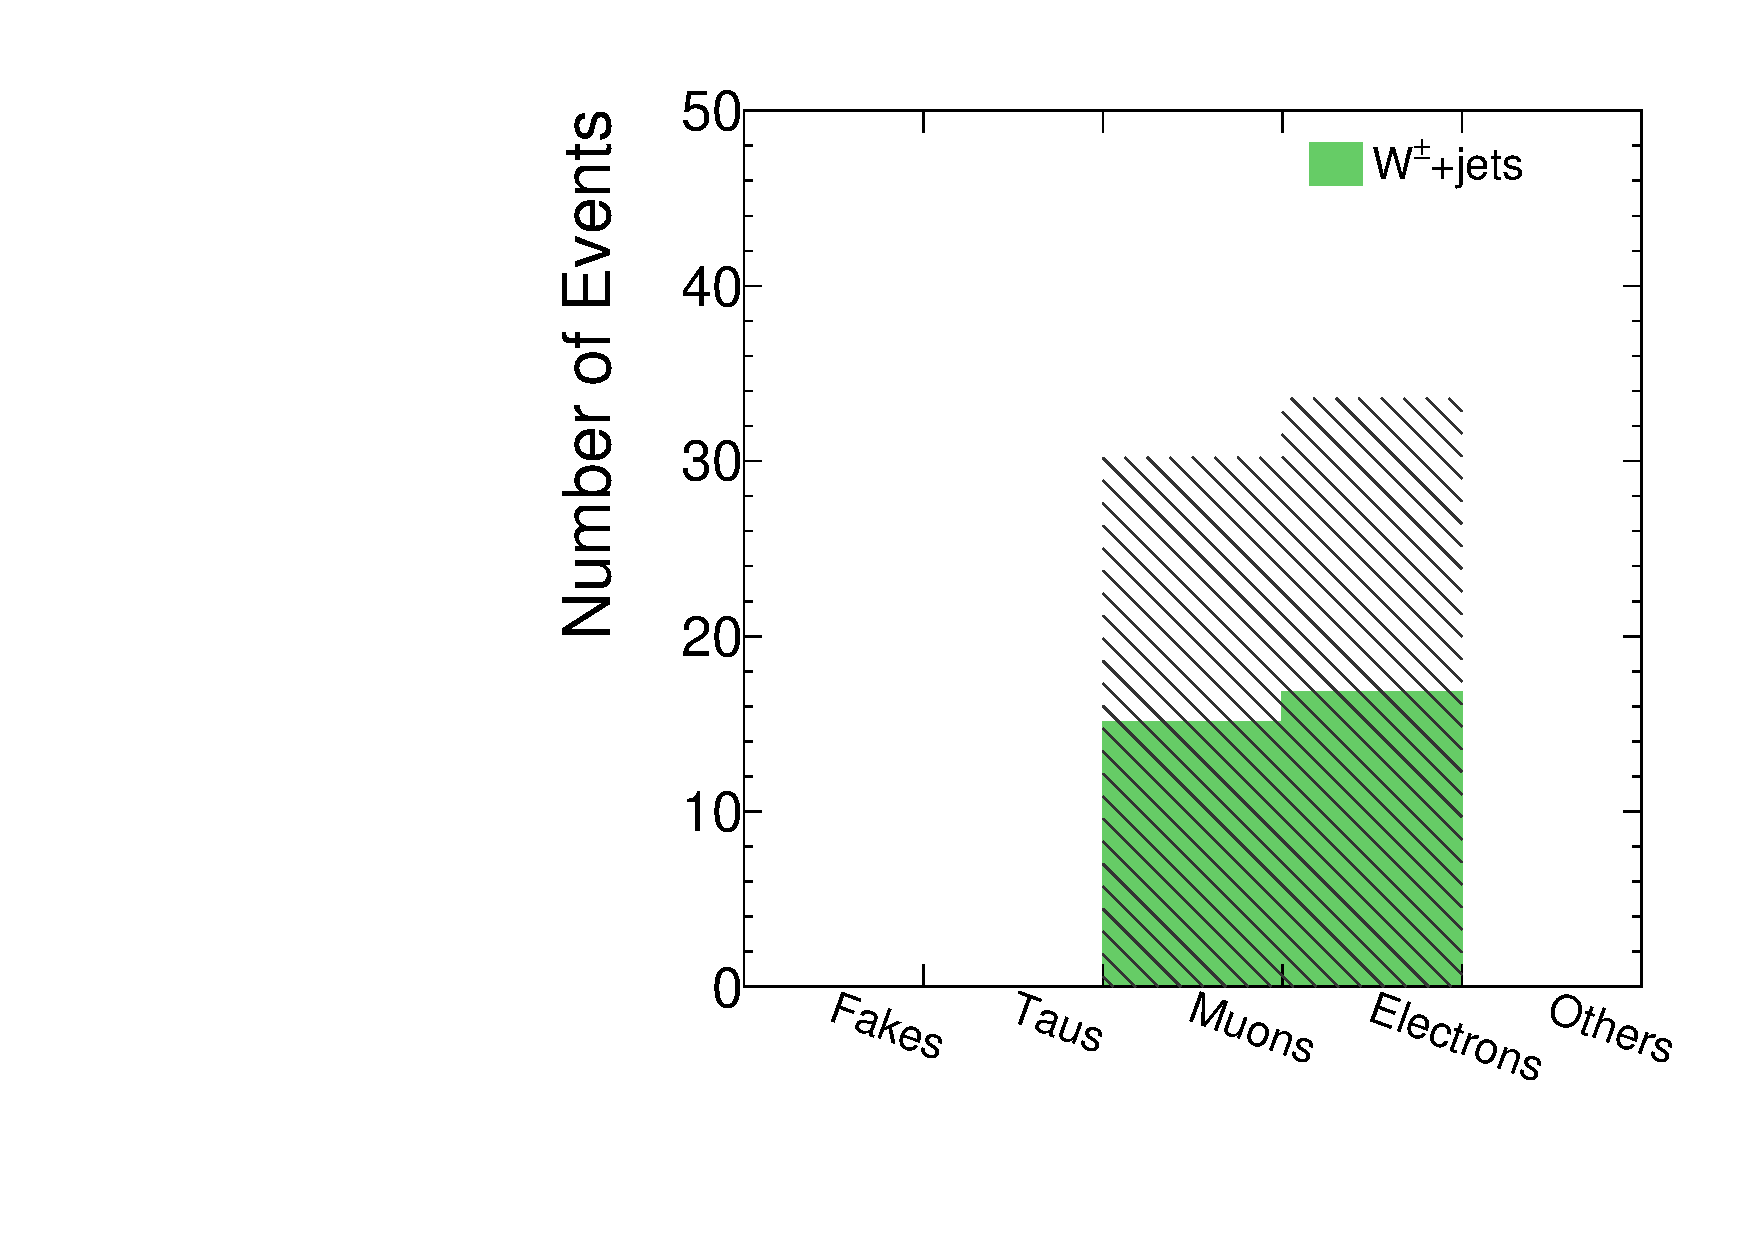
\includegraphics[width=0.49\textwidth]{figures/analysis/AnalysisSelection/chiTracksfullSelectionTrigger_Wjets/htrackgenParticleSmallRange_lin.pdf}
    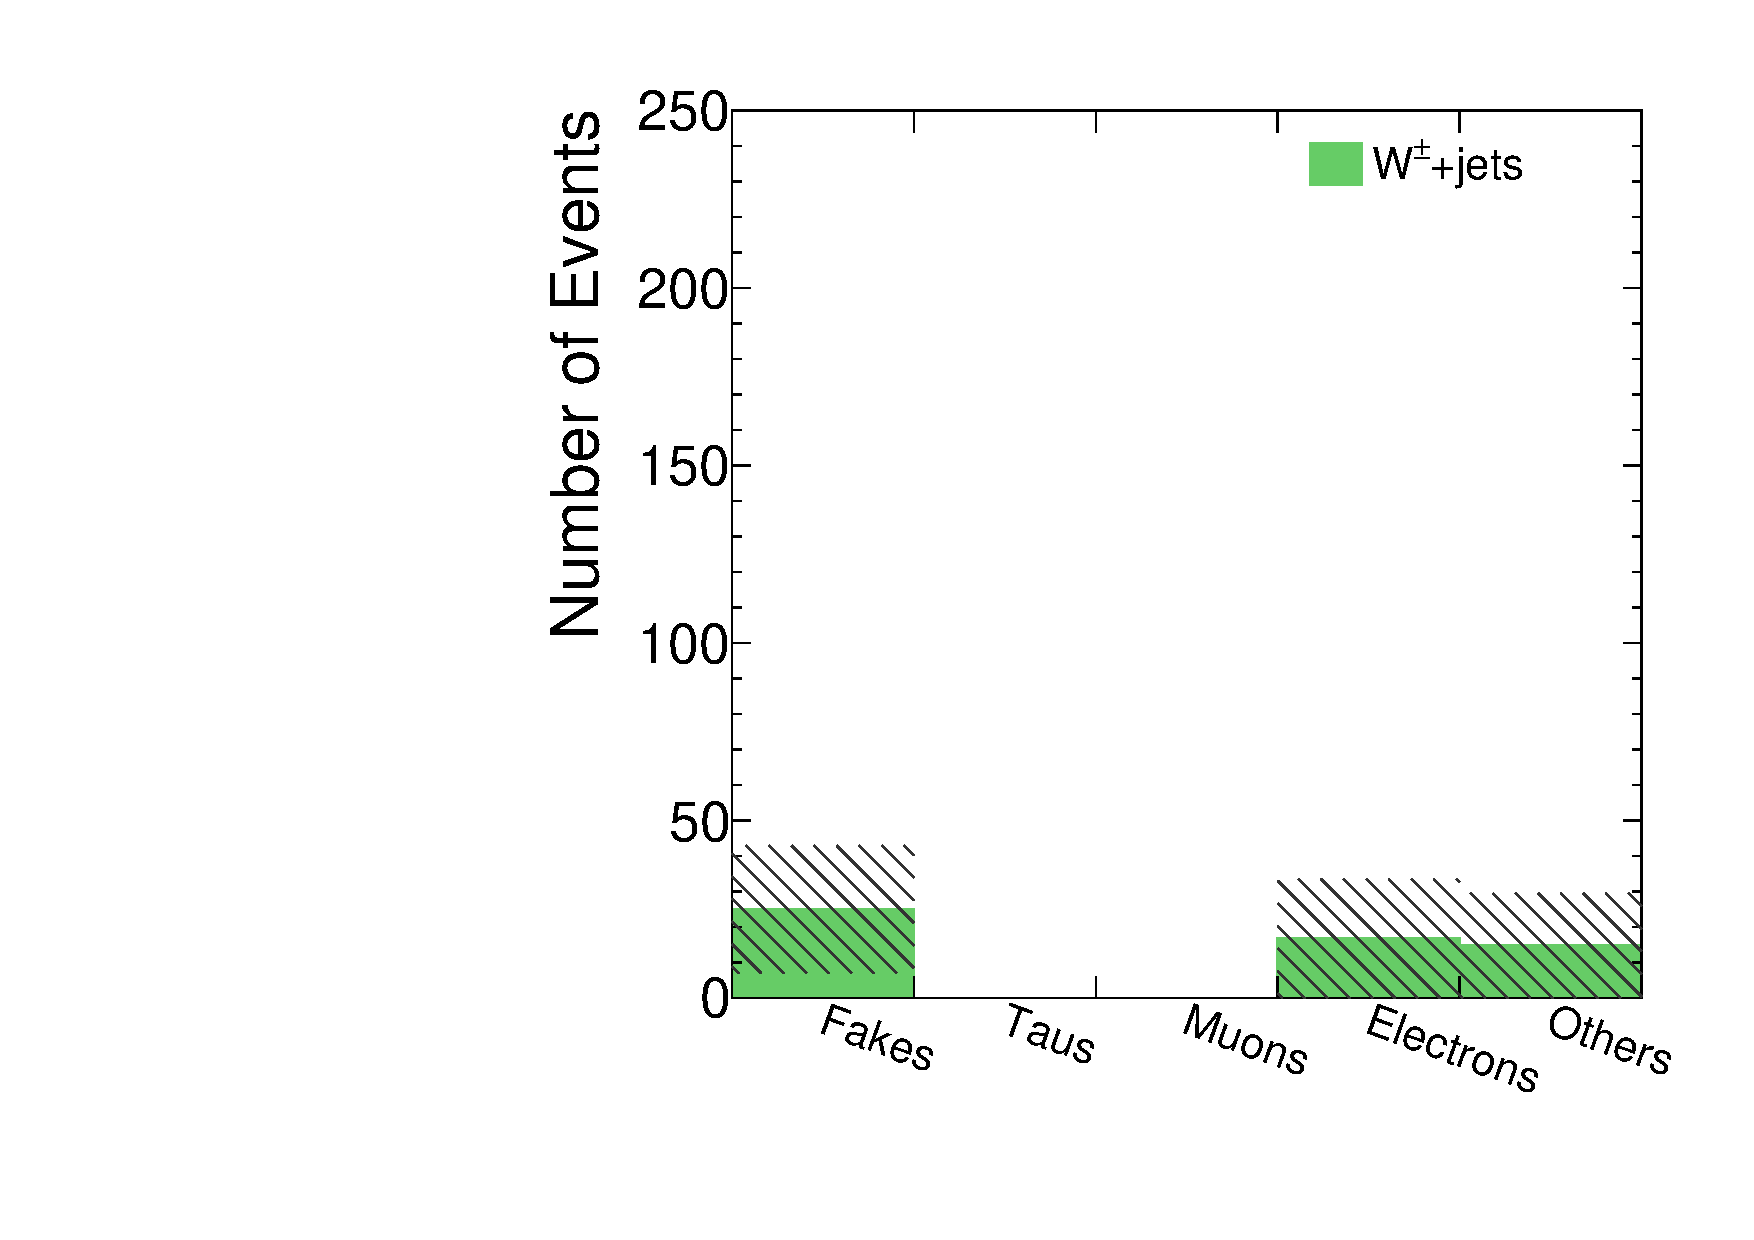
\includegraphics[width=0.49\textwidth]{figures/analysis/AnalysisSelection/chiTracksfullSelectionPlusIasTrigger_Wjets/htrackgenParticleSmallRange_lin.pdf}
  \end{tabular}
  \caption{Background composition in the simulated \WJets dataset after the full candidate track selection (left) and after the full candidate track selection plus an additional selection cut of \mbox{$\ias>0.05$} (right). 
           The statistical uncertainty is depicted by the hashed grey area.
           Given the limited size of the simulated \WJets dataset, the uncertainty of the composition is accordingly large.}
  \label{fig:BkgComposition}
\end{figure}
This composition can change significantly when imposing further selection cuts on \pt and \ias.
The definition of the signal region will be, however, addressed within the optimisation of the search sensitivity in Section~\ref{sec:Optimisation}.
To get a feeling how the composition of the background is affected by further cuts on one of the main variables, 
the background composition is also shown with the candidate track selection plus an additional \ias cut of 0.05.
It can be seen that the fake background is less reduced by an additional selection cut on \ias.
This gains even more in importance when considering all sources of fake tracks.
The fake background is not only present in \WJets events but essentially in all Standard Model processes.\\

Still, also the leptonic background can be important.
Unfortunately, because of the limited size of the simulated \WJets dataset, it is not possible to study the leptonic contribution to the background with simulated events.
Furthermore, when the simulation of the operativeness of every single detector module is not fully correct, the simulation could highly underestimate the leptonic background.\\

Therefore, a data-based approach is needed for either of the two background sources: the fake and the leptonic background.
%%%%%%%%%%%%%%%%%%%%%%%%%%%%%%%%%%%%%%%%%%%%%%%%%%%%%%%%%%%%%%%%%%%%%%%%%%%%%%%%%%%%%%%%%%%%%%%%%%%%%%%%%%%%%%%%%%%%%%%%%%%%%%%%%%%%%%%%%%%%%%%%%%%%%%%%%%%%%%%%%%%%%%%%%%%%%%%%%%%%
%%%%%%%%%%%%%%%%%%%%%%%%%%%%%%%%%%%%%%%%%%%%%%%%%%%%%%%%%%%%%%%%%%%%%%%%%%%%%%%%%%%%%%%%%%%%%%%%%%%%%%%%%%%%%%%%%%%%%%%%%%%%%%%%%%%%%%%%%%%%%%%%%%%%%%%%%%%%%%%%%%%%%%%%%%%%%%%%%%%%
\section{Fake background}
\label{sec:FakeBkg}
Fake tracks are tracks which are not reconstructed out of the trajectory of one single particle.
The rate with which this wrong reconstruction occurs is of course highly restrained by the quality cuts on $\chi^2$ and the vertex compatibility of the track reconstruction algorithm.
Details on the reconstruction algorithm at CMS can be found in Section~\ref{FIXME}.
The probability of reconstructing a fake track is strongly correlated with the number of hits in the tracker system.
This can be seen in Fig~\ref{fig:NValidFakes}, where the distribution in the number of hits of fakes is depicted.
\begin{figure}[!bt]
  \centering 
  \begin{tabular}{c}
    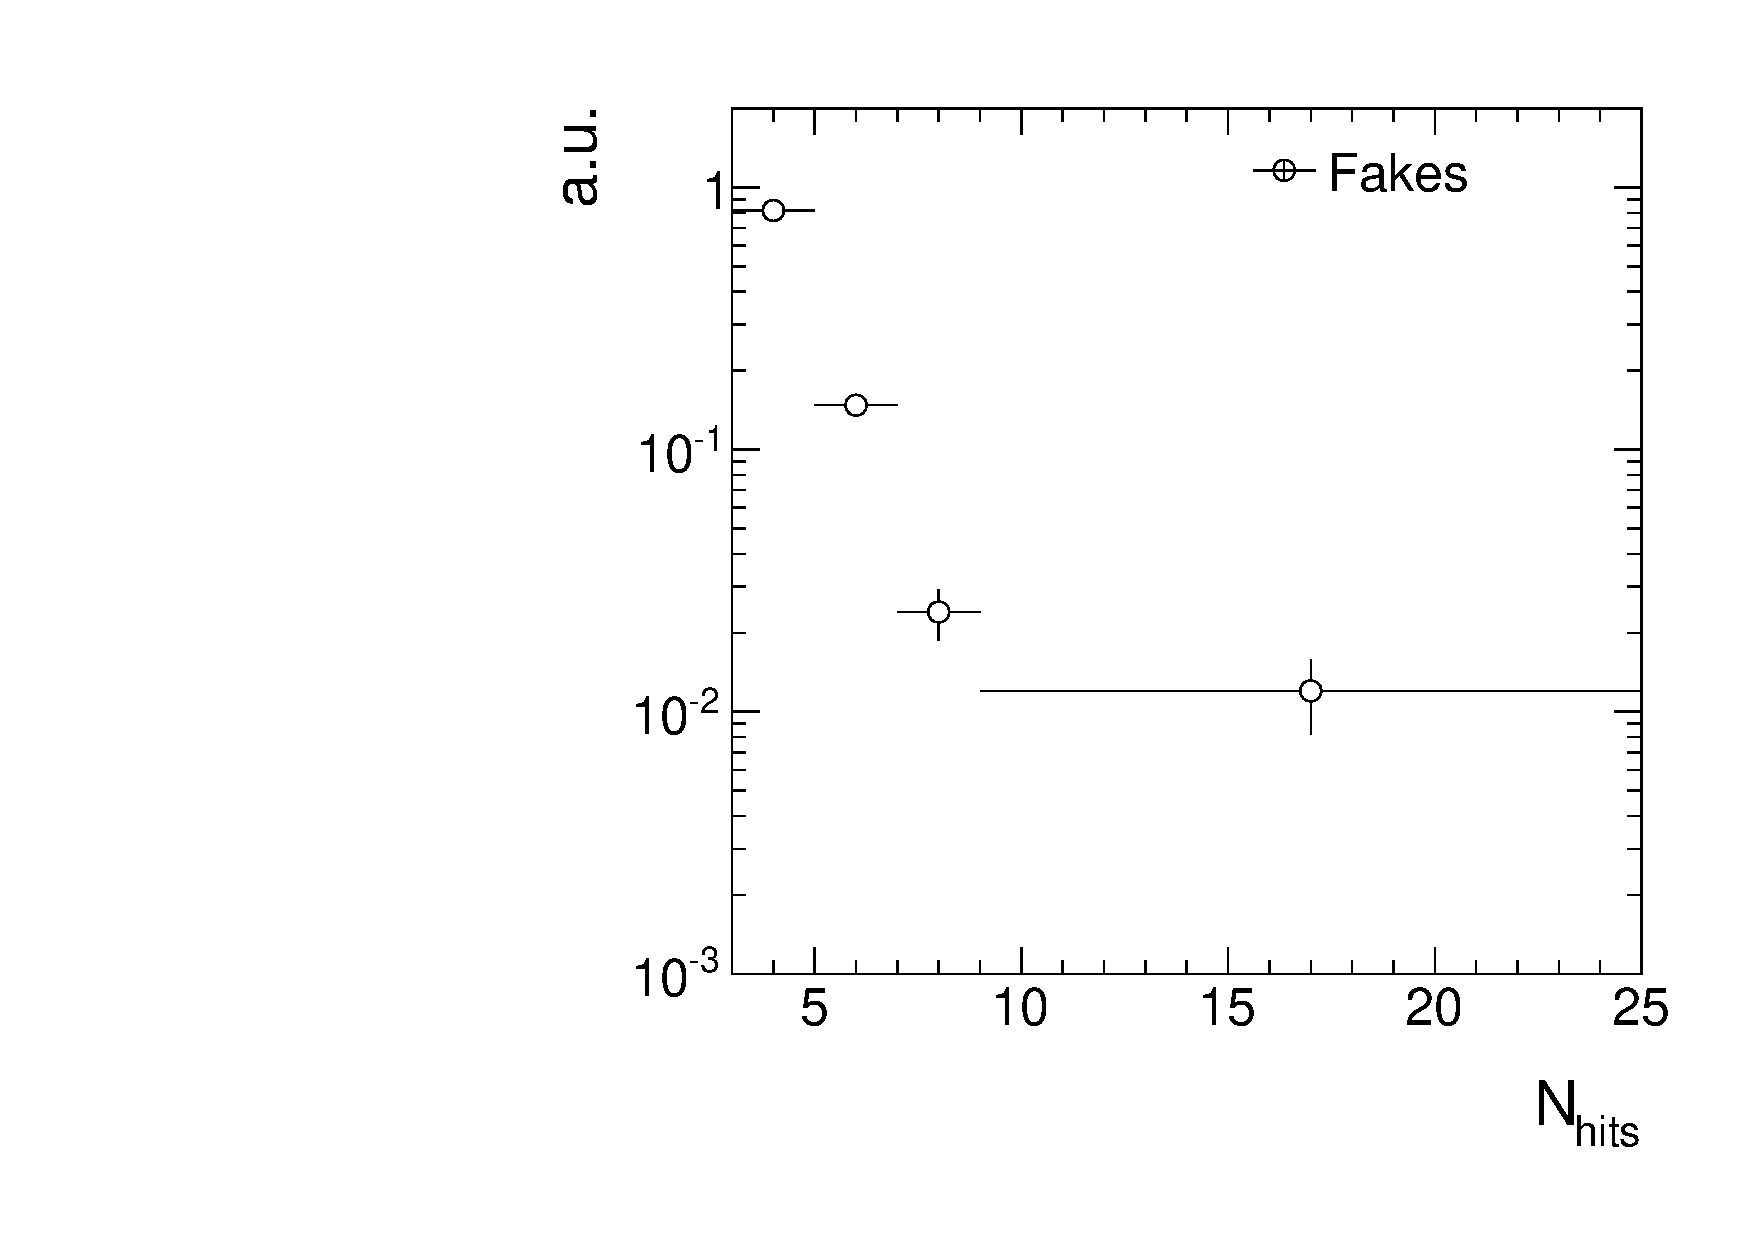
\includegraphics[width=0.49\textwidth]{figures/analysis/NValidForFakes_chiTracksfullSelectionNoQCDCutsNoTrigger_PtGt15GeV.pdf}
  \end{tabular}
  \caption{Normalised distribution of the number of hits for fake tracks.}
  \label{fig:NValidFakes}
\end{figure}
There are almost no fakes with a number of hits larger than six.
In simulation, fake tracks are defined as tracks which cannot be matched to a generator-level particle within a distance of $\Delta R < 0.01$.

Fakes are efficiently suppressed by the requirements of no missing middle or inner hits and the compatibility with the primary vertex.
Unfortunately, wrongly reconstructed tracks which pass these criteria, do also easily pass the $\ecalo<5\gev$ requirement with high efficiency.\\

In this analysis, the estimation of the fake background is split into two parts.
First, the background is estimated inclusively in \ias.
Second, to be able to optimise later in the variable \ias, the \ias distribution is taken from a fake enriched control region.

\subsection*{Inclusive fake background estimation}
The inclusive background estimation follows closely the background estimation method done in~\cite{bib:CMS:DT_Thesis,bib:CMS:DT_8TeV_AN}.
It aims to determine the probability of having a fake track in an event that pass the full track selection (besides the \ias criterium).
This probability will be called the fake rate.

The inclusive fake background is estimated with the help of $Z\rightarrow\mu\bar{\mu}$ and $Z\rightarrow e\bar{e}$ events from data.
Selecting clean \Zlep events can be done with high efficiency by requiring two well reconstructed muons or electrons, that are opposite in charge and for which the invariant mass is around the $Z$-boson mass of $\sim90\gev$.
Putting on top the candidate track selection described in Section~\ref{sec:CandidateTrackSelection}, the selected track must be a fake.

The selection of two well reconstructed muons and electrons is done with the single-muon and single-electron datasets listed in Table~\ref{tab:ElectronMuonCRDatasets}.
\renewcommand{\arraystretch}{1.5}
\begin{table}[!hbt]
\centering
\caption{Datasets used for the determination of the fake rate.}
\label{tab:ElectronMuonCRDatasets}
\makebox[0.99\textwidth]{
\begin{tabular}{lr}
\multicolumn{2}{c}{} \\
\toprule
Dataset  & Luminosity [\fbinv]   \\
\midrule
/SingleMu/Run2012A-22Jan2013-v1/AOD        &  0.876 \\
/SingleMu/Run2012B-22Jan2013-v1/AOD        &  4.405 \\
/SingleMu/Run2012C-22Jan2013-v1/AOD        &  7.040 \\
/SingleMu/Run2012D-22Jan2013-v1/AOD        &  7.369 \\ 
\midrule
/SingleElectron/Run2012A-22Jan2013-v1/AOD  &  0.876 \\
/SingleElectron/Run2012B-22Jan2013-v1/AOD  &  4.412 \\
/SingleElectron/Run2012C-22Jan2013-v1/AOD  &  7.050 \\
/SingleElectron/Run2012D-22Jan2013-v1/AOD  &  7.368 \\
\bottomrule
\end{tabular}}
\end{table}  
For the $Z\rightarrow\mu\bar{\mu}$ selection an event is required to have two muons with $\pt>25\gev$ and $|\eta|<2.4$.
To supress background from cosmic muons, the distance from the primary vertex must be less than $|d0|<0.2\cm$ in radial and $|dz|<0.5\cm$ in longitudinal direction.
To supress background arising from jets that fake muons, various quality criteria are apllied. 
Thus, it is required that there is at least one hit in the muon detector and at least two hits in different detector planes.   
Concerning the track of the muon in the tracker system, at minimum one hit in the pixel tracker and at least six hits in the full tracker system is required. 
An isolation criterium is applied that requires the sum of transverse momenta in a cone of $\Delta R<0.4$ of all PF particles to be less than 12\%.
Finally, the muons are required to be opposite in charge and that their invariant mass is between $80-100\gev$.
The $Z\rightarrow\mu\bar{\mu}\,+\,\text{fake track}$ selection is summarised in Table~\ref{tab:FakeMuonSample}.
\renewcommand{\arraystretch}{1.4}
\begin{table}[!h]
\centering
\caption{Event selection cuts for the muon control sample to estimate the inclusive fake background.}
\label{tab:FakeMuonSample}
\makebox[0.99\textwidth]{
\begin{tabular}{l|l l }
\multicolumn{3}{c}{} \\
\toprule
\multirow{12}{*}{\makecell[l]{Event based \\ selection}}       &  Two global muons with & $\pt>25\gev$ \\
                                                               &                        & $|\eta|<2.4$ \\
                                                               &                        & $\sum\limits_{\Delta R<0.4} \pt^{\text{PF particle}}/\pt(\mu)<0.12$ \\
                                                               &                        & $\left.\frac{\chi^2}{ndof}\right\rvert_{\text{global track}}<10$ \\
                                                               &                        & $|d0|<0.2\cm$  \\
                                                               &                        & $|dz|<0.5\cm$  \\
                                                               &                        & $\geq$ 1 hit in the muon detector  \\
                                                               &                        & $\geq$ 2 hits in different muon detector planes  \\
                                                               &                        & $\geq$ 1 hit in the pixel detector  \\
                                                               &                        & $\geq$ 6 hits in the tracker system  \\
                                                               &  \multicolumn{2}{l}{Muons opposite in charge}                                     \\
                                                               &  \multicolumn{2}{l}{$80\gev<M_{\text{inv}}\left(\mu_1,\mu_2  \right)<100\gev$}        \\

\midrule

\multirow{4}{*}{\makecell[l]{Candidate track\\ selection}}    &  Good quality selection \\
                                                              &  Kinematic selection    \\
                                                              &  Lepton/jet veto        \\   
                                                              &  Isolation selection    \\  
\bottomrule
\end{tabular}}
\vspace{10pt}
\end{table}

In order to select $Z\rightarrow e\bar{e}$ events in data, the two electrons are required to have \mbox{$\pt>25\gev$}, $|\eta|<2.5$ and no missing hits in the inner layers of the tracker.
Furthermore, the electrons need to pass a conversion veto to reduce background arising from photon conversions (as described in~\cite{bib:CMS:ConversionVeto_PAS}).
An isolation requirement is applied similar to the muon isolation criterium with a reduced cut of 15\%.
The electron identification is further based on a multivariate technique developed within~\cite{bib:CMS:ElectronMVA} that exploits electron characteristics about the track quality, the ECAL cluster shapes, and the combination about the measurements in the tracker and in the ECAL.
Again, also the two electrons must be opposite in charge and their invariant mass must be between $80-100\gev$.
A summary of the $Z\rightarrow e\bar{e}\,+\,\text{fake track}$ event selection can be found in Table~\ref{tab:FakeElectronSample}.\\
\renewcommand{\arraystretch}{1.4}
\begin{table}[!h]
\centering
\caption{Event selection cuts for the electron control sample to estimate the inclusive fake background.}
\label{tab:FakeElectronSample}
\makebox[0.99\textwidth]{
\begin{tabular}{l|l l }
\multicolumn{3}{c}{} \\
\toprule
\multirow{8}{*}{\makecell[l]{Event based \\ selection}}        &  Two Electrons with    & $\pt>25\gev$ \\
                                                               &                        & $|\eta|<2.5$ \\
                                                               &                        & $\sum\limits_{\Delta R<0.4} \pt^{\text{PF particle}}/\pt(e)<0.15$ \\
                                                               &                        & pass conversion veto    \\
                                                               &                        & no missing tracker hits  \\
                                                               &                        & good MVA electron as defined in \cite{bib:CMS:ElectronMVA}  \\
                                                               &  \multicolumn{2}{l}{Electrons opposite in charge}                                     \\
                                                               &  \multicolumn{2}{l}{$80\gev<M_{\text{inv}}\left(e_1,e_2  \right)<100\gev$}        \\

\midrule

\multirow{4}{*}{\makecell[l]{Candidate track\\ selection}}    &  Good quality selection \\
                                                              &  Kinematic selection    \\
                                                              &  Lepton/jet veto        \\   
                                                              &  Isolation selection    \\  
\bottomrule
\end{tabular}}
\end{table}  

When applying a \Zlep selection plus the candidate track selection, the selected track should be a fake.
If this is indeed the case can be tested on simulated \Zlep events.
As can be seen in Fig.~\ref{fig:BkgComposition}, a reasonable purity in fake tracks can be achieved by applying the candidate track selection on top of the \Zlep selection.
In simulated $Z\rightarrow\mu\bar{\mu}$ events, a purity of 88\%, whereas in simulated $Z\rightarrow e\bar{e}$ events a purity of 92\% of fake tracks can be achieved.


As already mentioned, the fake rate is defined as the probability that an event contains a fake track that fulfils the candidate track selection criteria listed in Section~\ref{sec:CandidateTrackSelection}.
Thus, for the \Zlep datasets it is defined as the number of events passing the full selection described in Table~\ref{tab:FakeMuonSample} (Table~\ref{tab:FakeElectronSample}) divided by the number of events that pass only the event based selection in Table~\ref{tab:FakeMuonSample} (Table~\ref{tab:FakeElectronSample})
\begin{equation*}
\rho_{\text{fake}} = \frac{N_{Z\rightarrow ll}^{\text{cand trk selection}}}{N_{Z\rightarrow ll}}
\end{equation*}
The fake rate for the candidate track selection is e.g. $\left( 8.75 \pm 0.28 \right) \cdot 10^{-5}$  (FIXME: update with correct pt cut). 
This is of course not the final result as the optimisation in \pt will add an additional \pt selection cut to the candidate track selection.
Within~\cite{bib:CMS:DT_Thesis,bib:CMS:DT_8TeV_AN}, it was checked that the fake rate is constant for different processes.
This is shown in Fig.~\ref{fig:FakeRate} where the fake rate is depicted for the most important SM processes.
\begin{figure}[!bt]
  \centering 
  \begin{tabular}{c}
    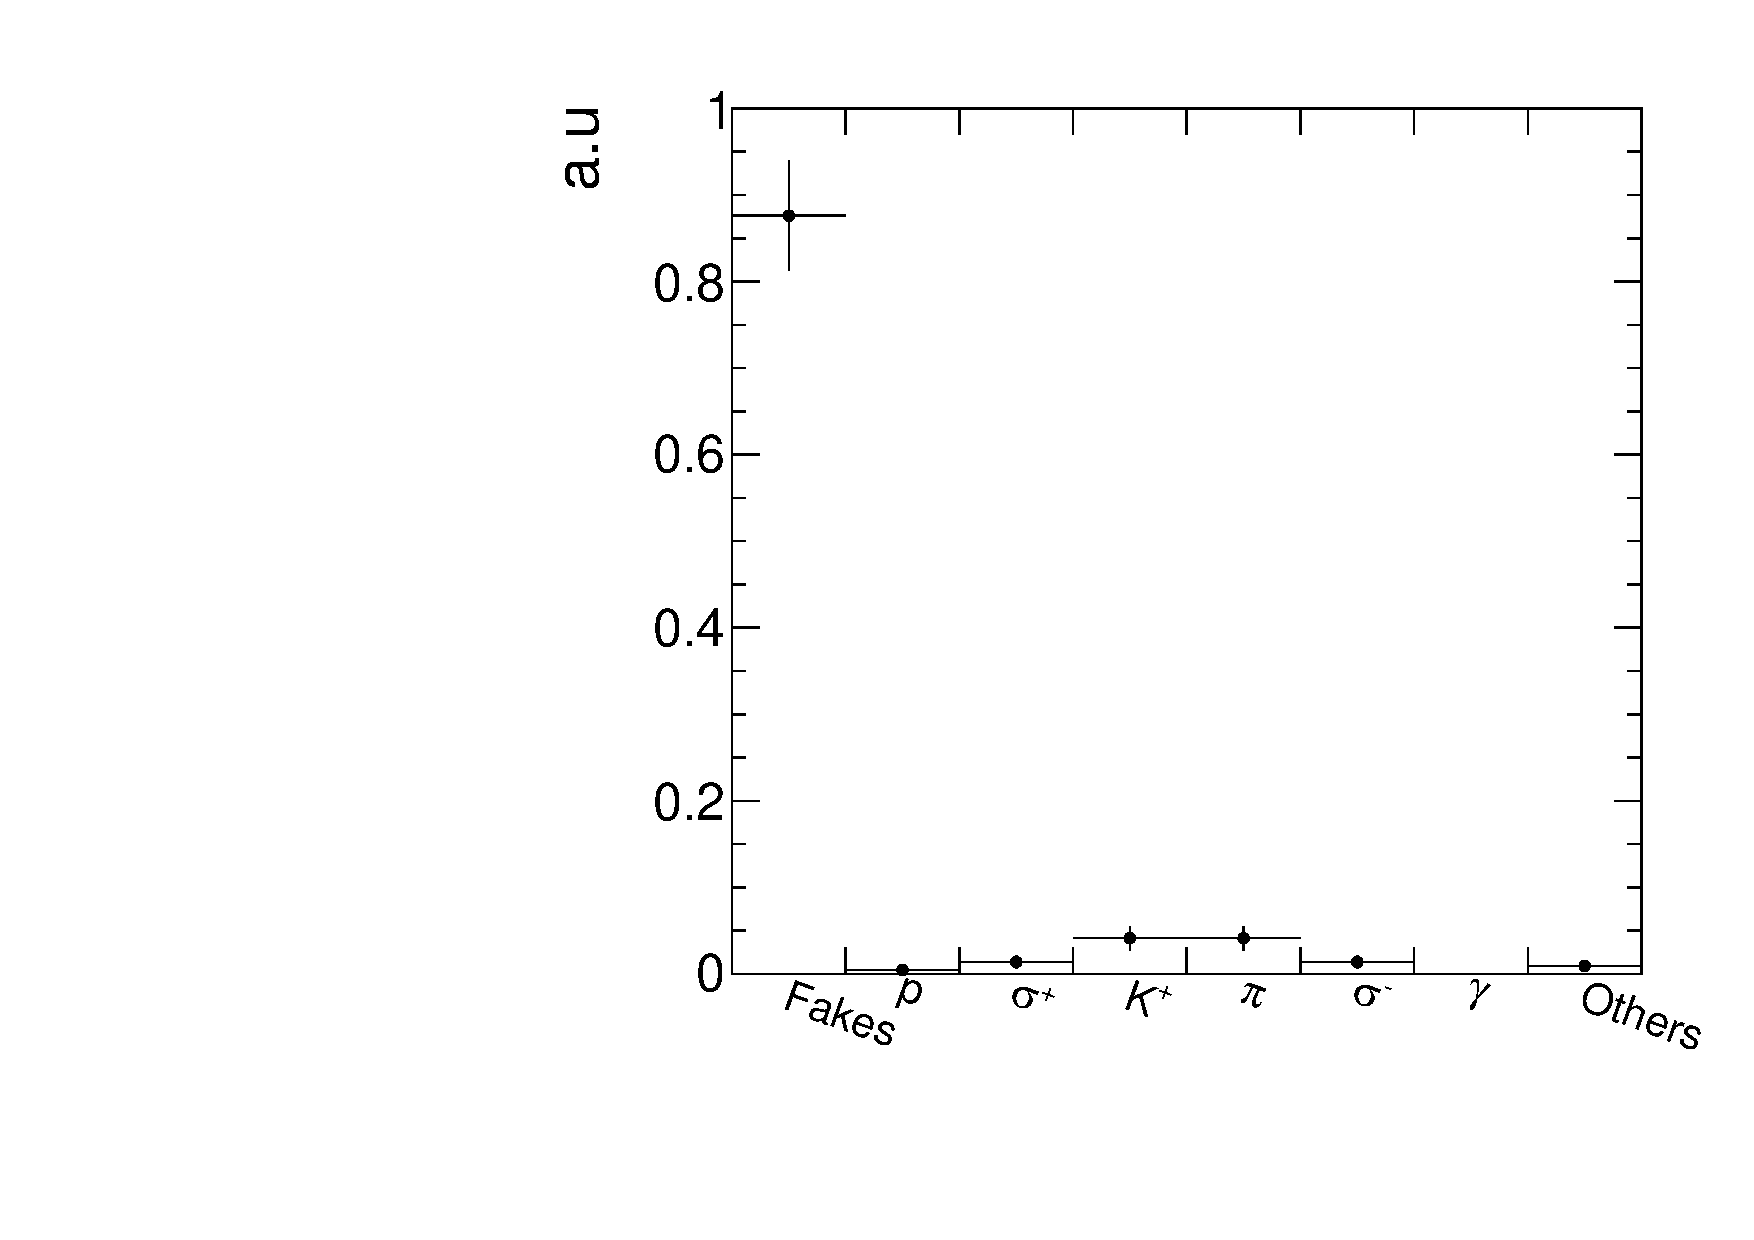
\includegraphics[width=0.49\textwidth]{figures/analysis/AnalysisSelection/ParticleCompositionInFakeCS_Mu.pdf}
    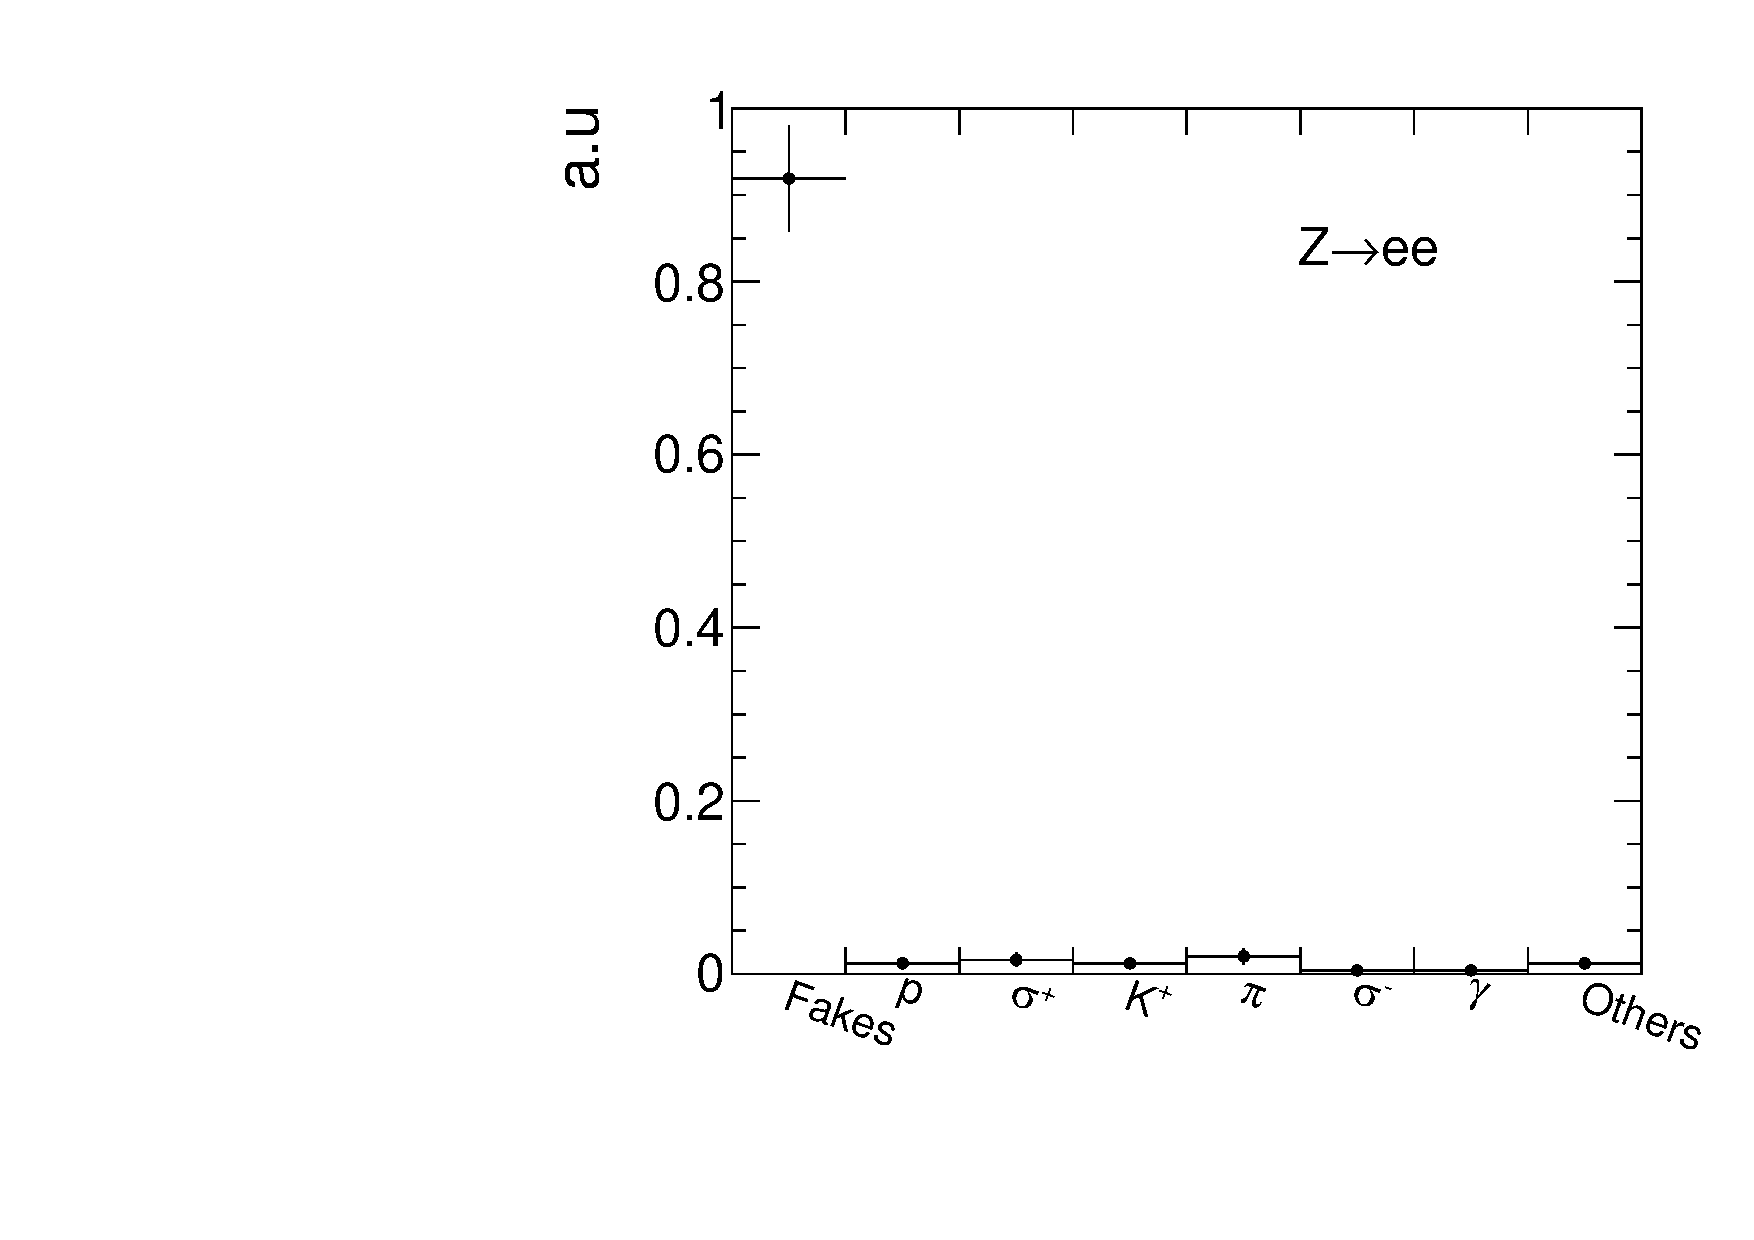
\includegraphics[width=0.49\textwidth]{figures/analysis/AnalysisSelection/ParticleCompositionInFakeCS_Ele.pdf}
  \end{tabular}
  \caption{Generator-level particle matched to the selected track with the selection described in Table~\ref{tab:FakeMuonSample} (left) and Table~\ref{tab:FakeElectronSample} (right). ``Fake'' mean that no corresponding generator-level particle could be found. }
\vspace{30pt}
  \label{fig:BkgComposition}
\end{figure}

\begin{figure}[!bt]
  \centering 
  \begin{tabular}{c}
    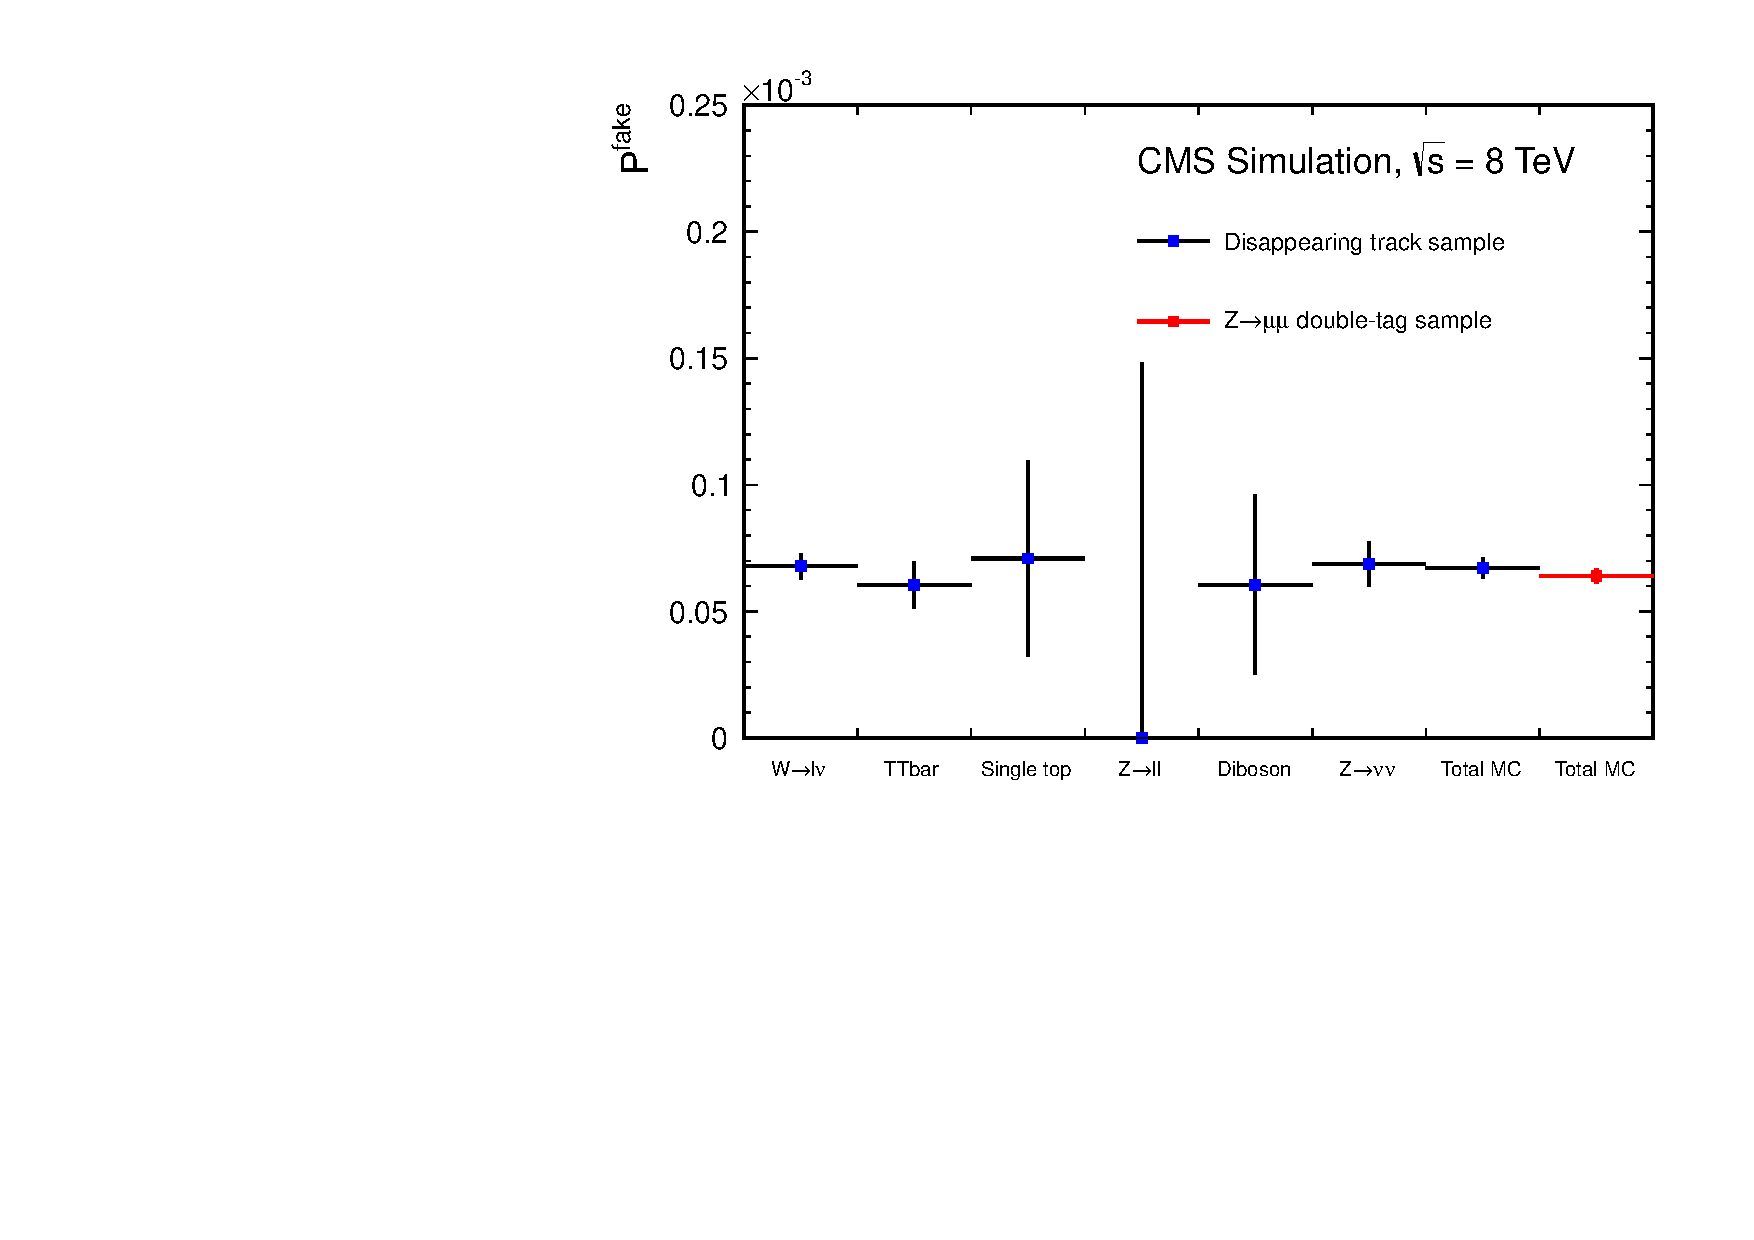
\includegraphics[width=0.79\textwidth]{figures/analysis/AnalysisSelection/fakeTrkRates.pdf}
  \end{tabular}
  \caption{Fake track rate estimated in \cite{bib:CMS:DT_Thesis,bib:CMS:DT_8TeV_AN} for tracks with four hits. Taken from \cite{bib:CMS:DT_8TeV_AN} }
  \label{fig:FakeRate}
\vspace{30pt}
\end{figure}

Since the fake rate is constant for different SM processes, the fake rate determined on the \Zlep dataset can be generalised for all SM background possibily contributing to this search.
Thus, the inclusive fake background can be estimated by multiplying the fake rate with the number of events selected in the MET dataset after the event based selection defined in Table~\ref{tab:SummaryCuts}
\begin{equation*}
N^{\text{fake, inclusive in I$_{\text{as}}$}}_{\text{bkg}} = \rho_{\text{fake}} \cdot N_{\text{event based selection}}^{\text{MET}}.
\end{equation*}
With a number of event after the event based selection in of $N_{\text{event based selection}}^{\text{MET}} = 1.38\cdot10^6$ and the fake rate cited above, 
the inclusive fake background can be e.g. estimated to $120.9\pm3.8$ for the candidate track selection.

It should again be mentioned that the inclusive fake background estimation will be only inclusive in \ias not in \pt.
That means that after the definition of the signal region, $N^{\text{fake, inclusive in I$_{\text{as}}$}}_{\text{bkg}}$ is determined with the additional optimal \pt selection.
To receive information about the selection efficiency of an \ias selection criterium, information about the \ias shape of fake tracks is needed.
How to get this, will be explained in the next section.

\subsection*{\ias shape of fake background}
Information of the energy release per path length for fake tracks should not be taken from simulated samples as the simulation of $dE/dx$ is not reliable (see Fig.~\ref{fig:Data-MC-Dedx_MIPs}).
To get still knowledge about the \ias shape of fake tracks, a control region needs to be defined that is enriched with fakes and shows the same \ias distribution as fake tracks in the signal region.

To enrich fake tracks, it is possible to invert the selection cuts of the number of missing middle and inner hits, i.e. requiring at least one missing inner or middle hit $\left( N_{\text{miss}}^{\text{inner}} +N_{\text{miss}}^{\text{middle}}>0\right)$ .
This can be seen in Fig~\ref{fig:NMissInnerAndMiddle}, where the distribution of the number of missing inner plus missing middle hits is shown for fakes compared to the leptonic background for simulated \WJets events.
Indeed, a high purity of around 90\% of fakes can be achieved for this definition of the \ias fake control region CR$_{\ias}^{\text{fake}}$.
\begin{figure}[!b]
  \centering 
  \begin{tabular}{c}
    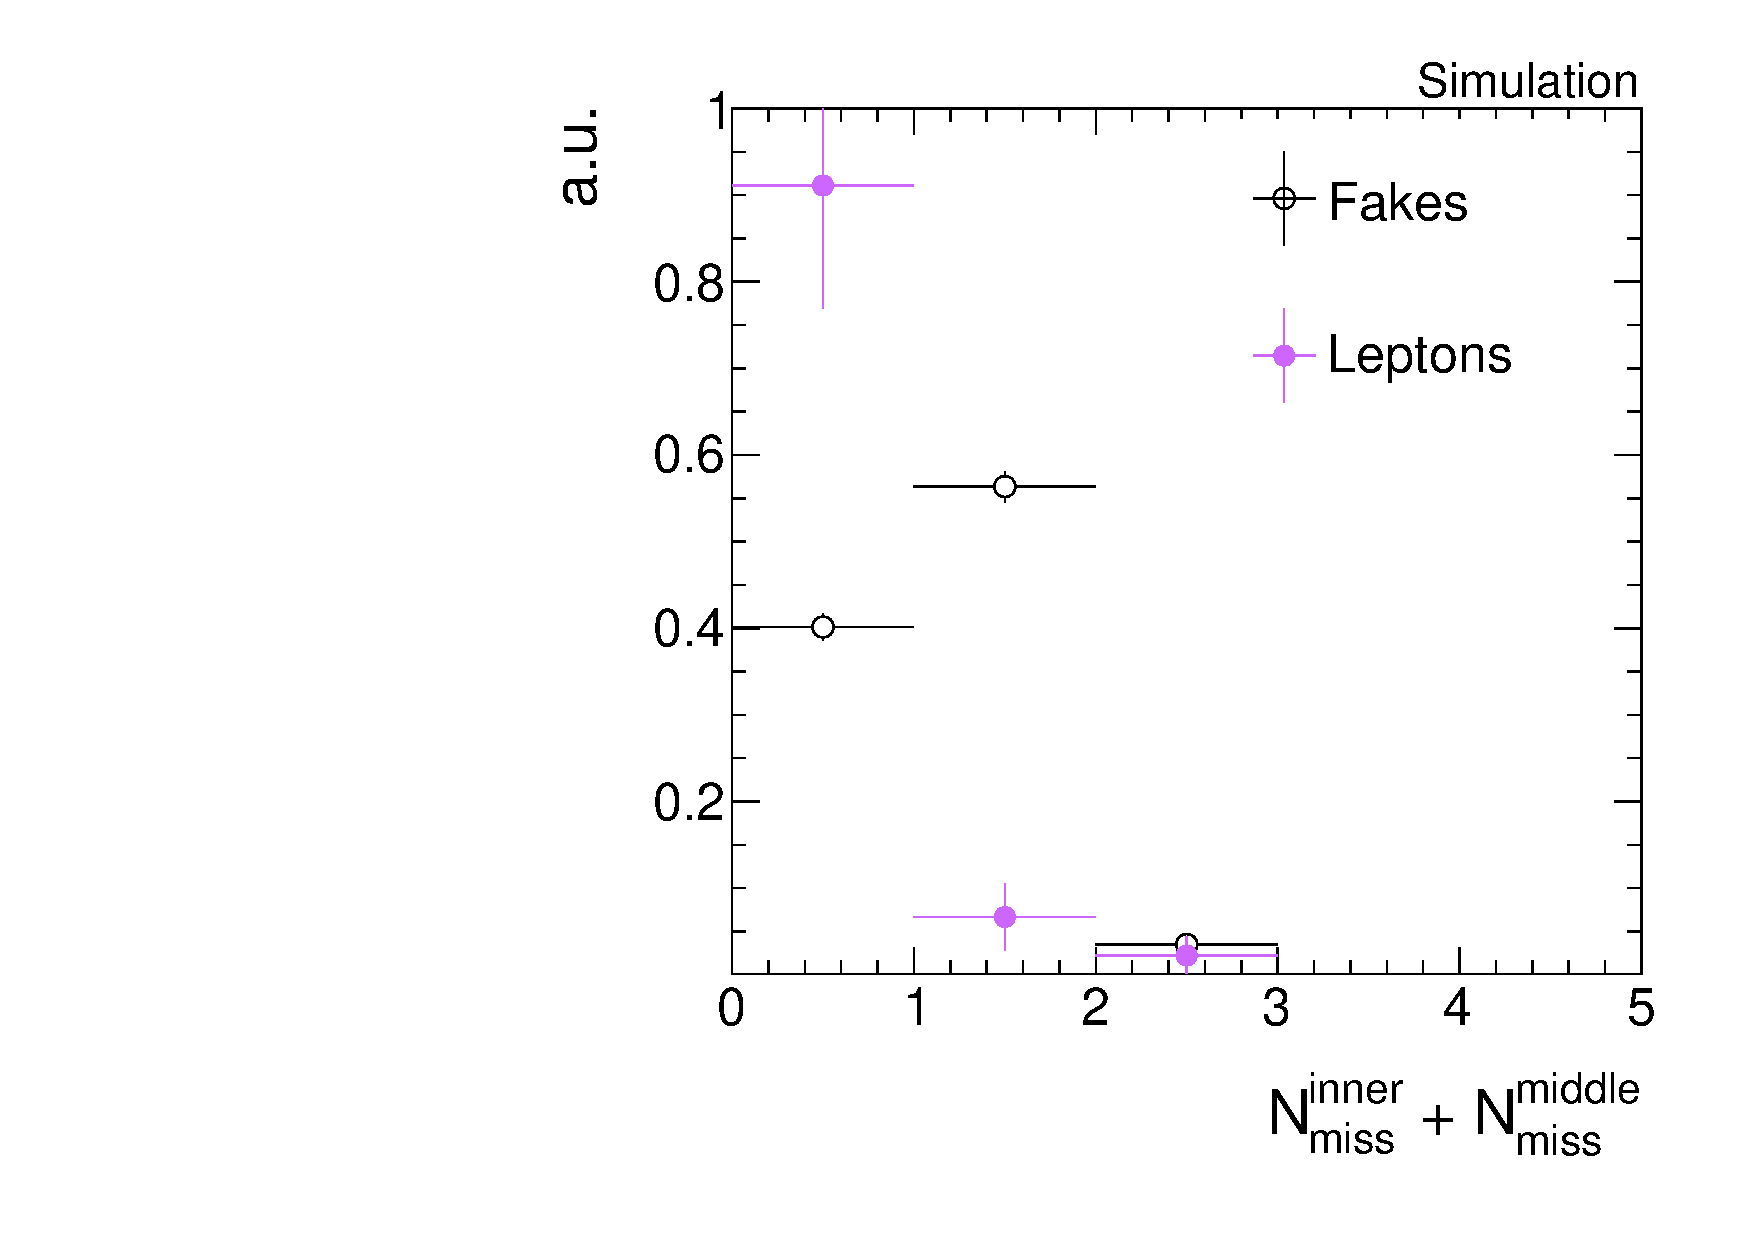
\includegraphics[width=0.49\textwidth]{figures/analysis/Background/NLostInnerPlusMiddleForAllBkg_chiTracksQCDsupressionTrigger.pdf}
  \end{tabular}
  \caption{Number of missing inner plus missing middle hits for fake and leptonic tracks for the full candidate track selection with the selection requirements on $N_{\text{miss}}^{\text{inner}}$ and $N_{\text{miss}}^{\text{middle}}$ removed.}
  \label{fig:NMissInnerAndMiddle}
\end{figure}

Of course, it needs also to be checked wether the \ias shape in CR$_{\ias}^{\text{fake}}$ is comparable to the \ias shape in the signal region.
As the exact definition of the signal region will be addressed during optimisation, this test will be done for various \pt selection cuts.

The comparison of the \ias shape of fake tracks can of course only be done on simulation.
Thus, simulated \WJets events are used to select fake tracks in both region.
A compariosn of the shape for the candidate track selection and the CR$_{\ias}^{\text{fake}}$ is shown in Fig~\ref{fig:IasSRCRFakes}.
\begin{figure}[!t]
  \centering 
  \begin{tabular}{c}
    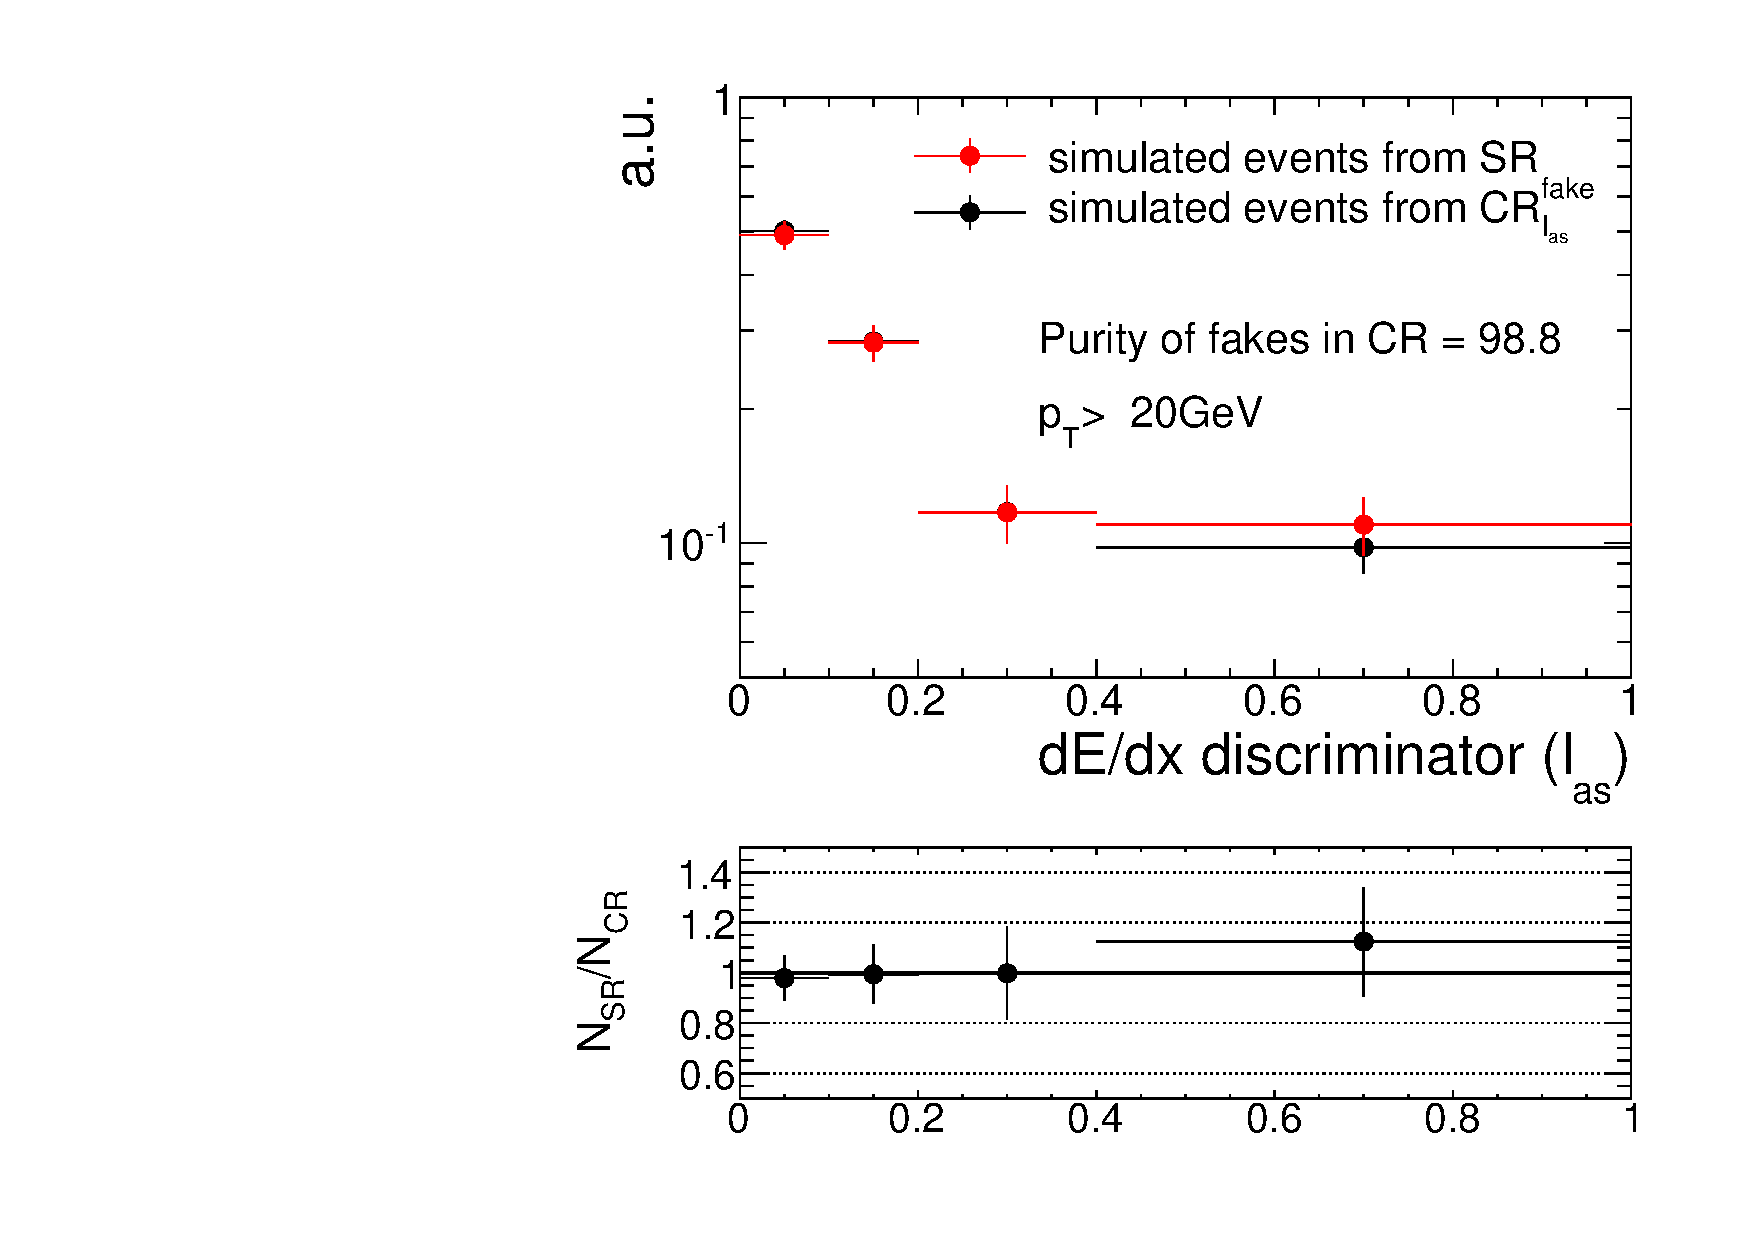
\includegraphics[width=0.49\textwidth]{figures/analysis/Background/hASmi_SRbinning_d0Inverted_fakes_ECalaoLe5_trackPtGt20_MC_CR_MC_SR.pdf}
    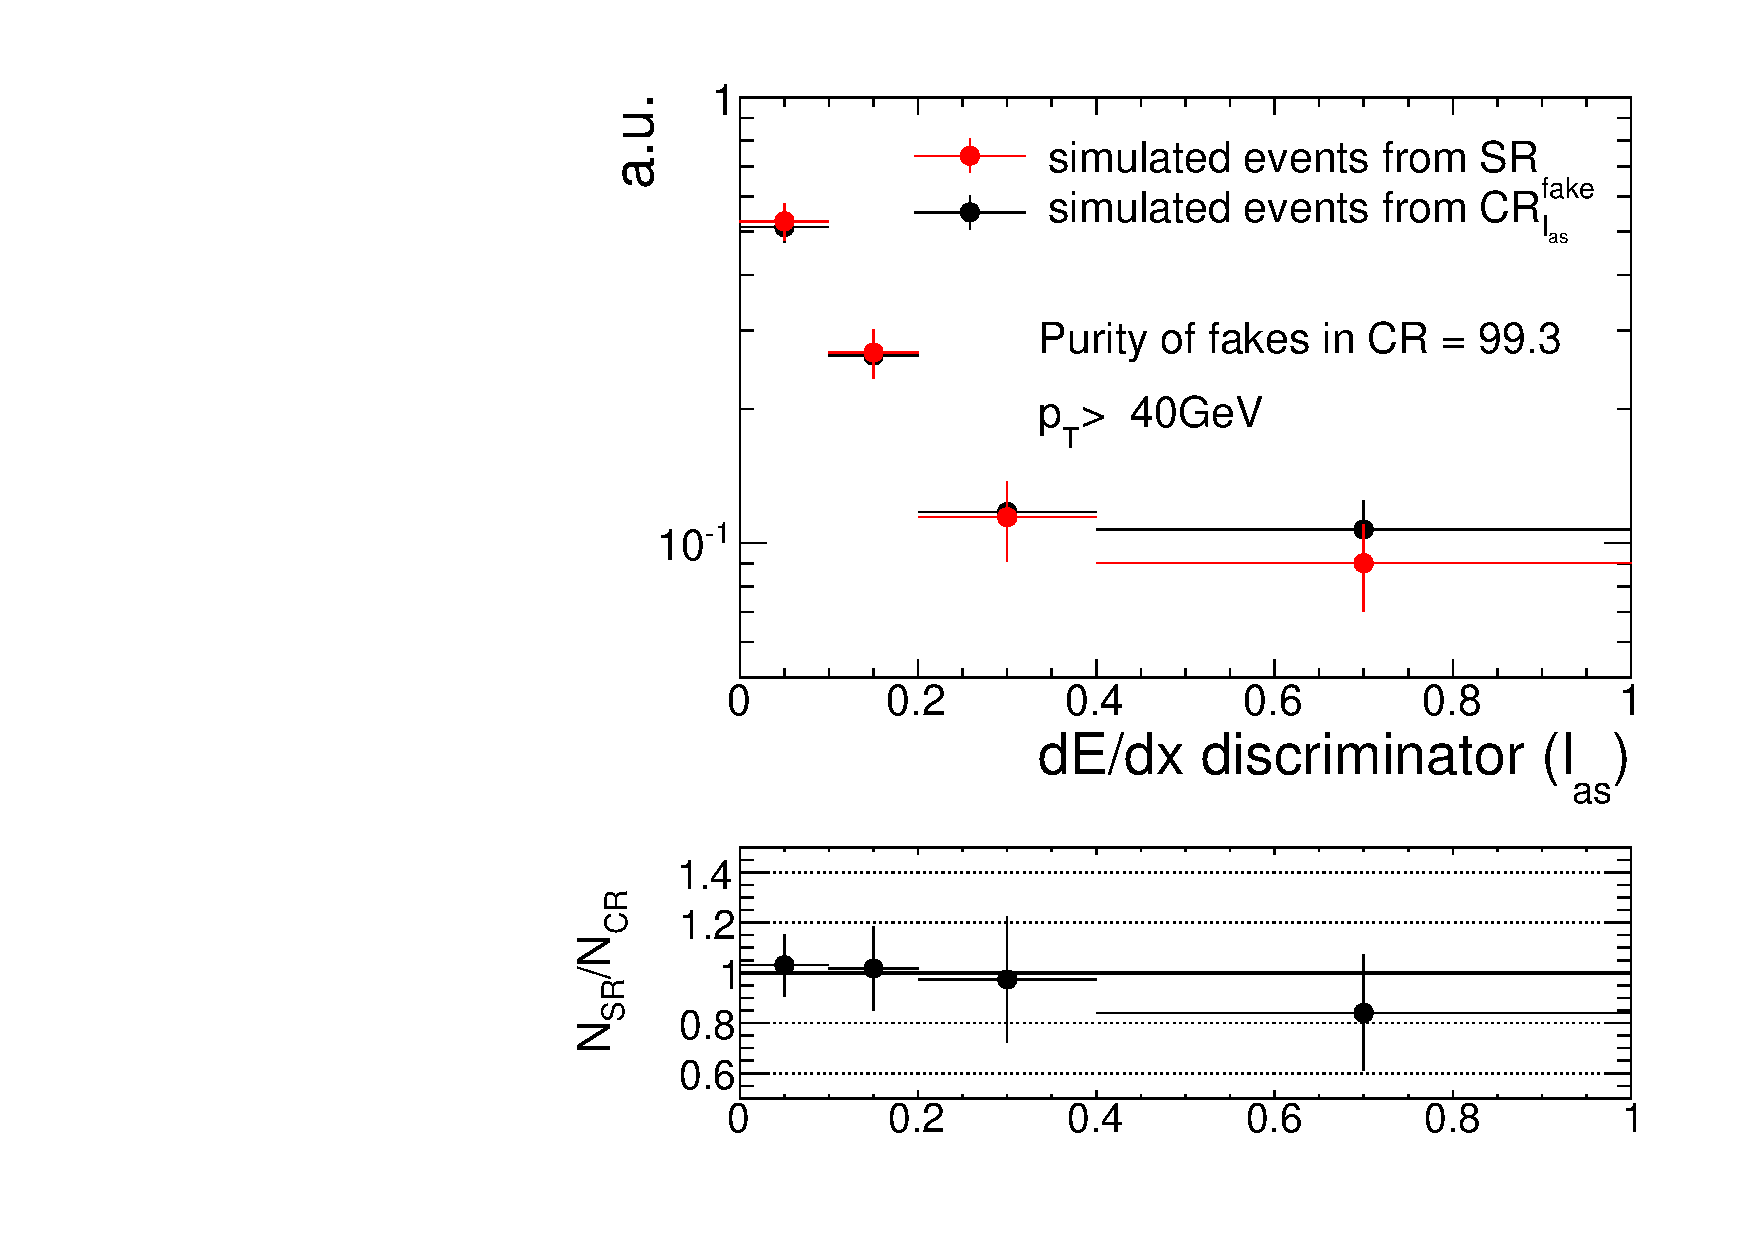
\includegraphics[width=0.49\textwidth]{figures/analysis/Background/hASmi_SRbinning_d0Inverted_fakes_ECalaoLe5_trackPtGt40_MC_CR_MC_SR.pdf}
  \end{tabular}
  \caption{Comparison of the \ias shape between CR$_{\ias}^{\text{fake}}$ and the signal region for two different track \pt cuts of 20\gev (left) and 40\gev (right). To enhance the statistical precision only the track selection is applied.}
  \label{fig:IasSRCRFakes}
\end{figure}

The \ias shape is almost identical in the signal and in the control region which makes the definition of the control region perfectly suited for the purpose to estimate the \ias shape from CR$_{\ias}^{\text{fake}}$ in data.
The differences between the both region will be taken as systematic uncertainty into account.
%%%%%%%%%%%%%%%%%%%%%%%%%%%%%%%%%%%%%%%%%%%%%%%%%%%%%%%%%%%%%%%%%%%%%%%%%%%%%%%%%%%%%%%%%%%%%%%%%%%%%%%%%%%%%%%%%%%%%%%%%%%%%%%%%%%%%%%%%%%%%%%%%%%%%%%%%%%%%%%%%%%%%%%%%%%%%%%%%%%%
%%%%%%%%%%%%%%%%%%%%%%%%%%%%%%%%%%%%%%%%%%%%%%%%%%%%%%%%%%%%%%%%%%%%%%%%%%%%%%%%%%%%%%%%%%%%%%%%%%%%%%%%%%%%%%%%%%%%%%%%%%%%%%%%%%%%%%%%%%%%%%%%%%%%%%%%%%%%%%%%%%%%%%%%%%%%%%%%%%%%
%%%%%%%%%%%%%%%%%%%%%%%%%%%%%%%%%%%%%%%%%%%%%%%%%%%%%%%%%%%%%%%%%%%%%%%%%%%%%%%%%%%%%%%%%%%%%%%%%%%%%%%%%%%%%%%%%%%%%%%%%%%%%%%%%%%%%%%%%%%%%%%%%%%%%%%%%%%%%%%%%%%%%%%%%%%%%%%%%%%%

\section{Leptonic background}
\label{sec:LeptonicBkg}

The leptonic background of the here presented search is caused by non-reconstructed leptons which undergo hence the lepton veto selection.
However, at least non-reconstructed electrons or taus should in principle deposit enough energy in the calorimeters such that they can still be vetoed by the calorimeter isolation requirement.
As muons don't deposit much energy in the calorimeters, this reason does not hold for them.
In the following, the sources of the three different leptonic backgrounds shall be characterised.

\subsection*{Electrons}
To avoid the background source from unreconstructed electrons, all tracks pointing to a dead or noisy ECAL cells are vetoed, as described in Section~\ref{sec:AnalysisSelection}.
By this selection, almost all electrons are efficiently rejected.
In the simulated \WJets sample only one simulated event remains that pass all candidate track selection criteria and where the candidate track can be matched to a generator-level electron.
This event is visualised in Fig~\ref{fig:LostElectron}. 
\begin{figure}[!tb]
  \centering 
  \begin{tabular}{c}
    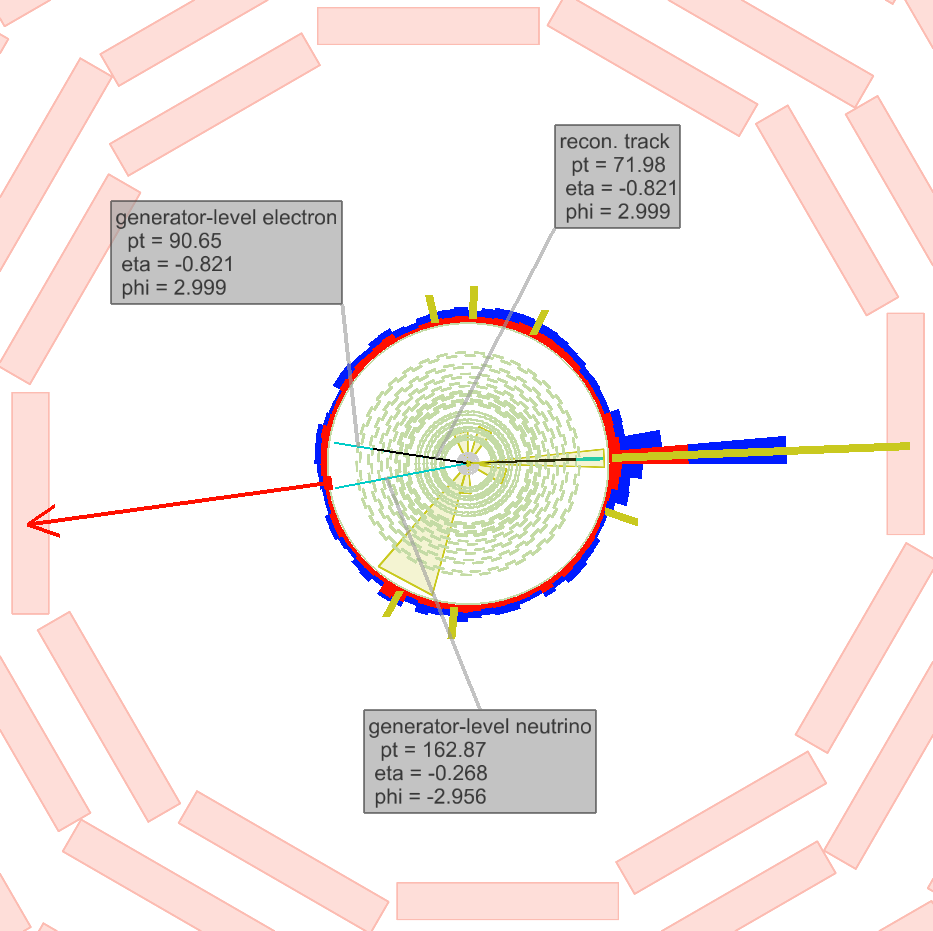
\includegraphics[width=0.49\textwidth]{figures/analysis/Electron_lumi_279317_event_111637553.png}
  \end{tabular}
  \caption{Visualisation of an $W\rightarrow e\nu_e$ event contributing to the SM background. 
           In light blue the generator-level particles $e$ and $\nu_e$ of the $W$ decay are shown. 
           The $\nu_e$, only weakly interacting does not show any signature in the detector, whereas the electron ($\pt\simeq 90\gev$) leaves a track (black line) with \mbox{$\pt\simeq 70\gev$} in the tracker. 
           No ECAL energy deposits in the direction of the electron are visible. 
           This is caused by the fact that the corresponding ECAL energy deposits were not read out in this event.
           An ISR jet ($\pt\simeq 230\gev$) causes the \met (read arrow) in the event. }
  \label{fig:LostElectron}
\end{figure}
In this event no energy deposits in the ECAL are read out, which suggests, that this ECAL tower was neither working properly in 2012.
Additionally, electrons can do bremsstrahlung which can change the direction of the electron significantly.
Thus, the energy deposits in the ECAL can possibly not be matched to the original electron.


\subsection*{Taus}
The tau background is contributing through the hadronic decay of a tau lepton to one charged pion $\tau\rightarrow\pi^{\pm}\nu$.
Unreconstructed taus are typically low energetic and can therefore bypass the calorimeter isolation criterion.
Because of nuclear interactions in the tracker, they can result in short reconstructed tracks which can easily be highly mismeasured in \pt.
Thus, pions can also contribute even when imposing a tighter selection in the transverse momentum.
Such an event is shown in Fig.~\ref{fig:LostTau}.


\subsection*{Muons}
Muons can fail reconstruction when they are pointing towards a bad cathode strip chamber.
This is taken into account in the candidate track selection.
However, some of the muons still fail reconstruction when they fall within the gap between stations 0 and 1 of the DT system at $|\eta|=0.25$.
The muon reconstruction efficiency drops from around 99\% to a value of around 94\% as shown in~\cite{bib:CMS:DT_Thesis,bib:CMS:DT_8TeV_AN}.
This possibility is illustrated in a simulated event shown in Fig~\ref{fig:LostMuon}.
\begin{figure}[!tb]
  \centering 
  \begin{tabular}{c}
    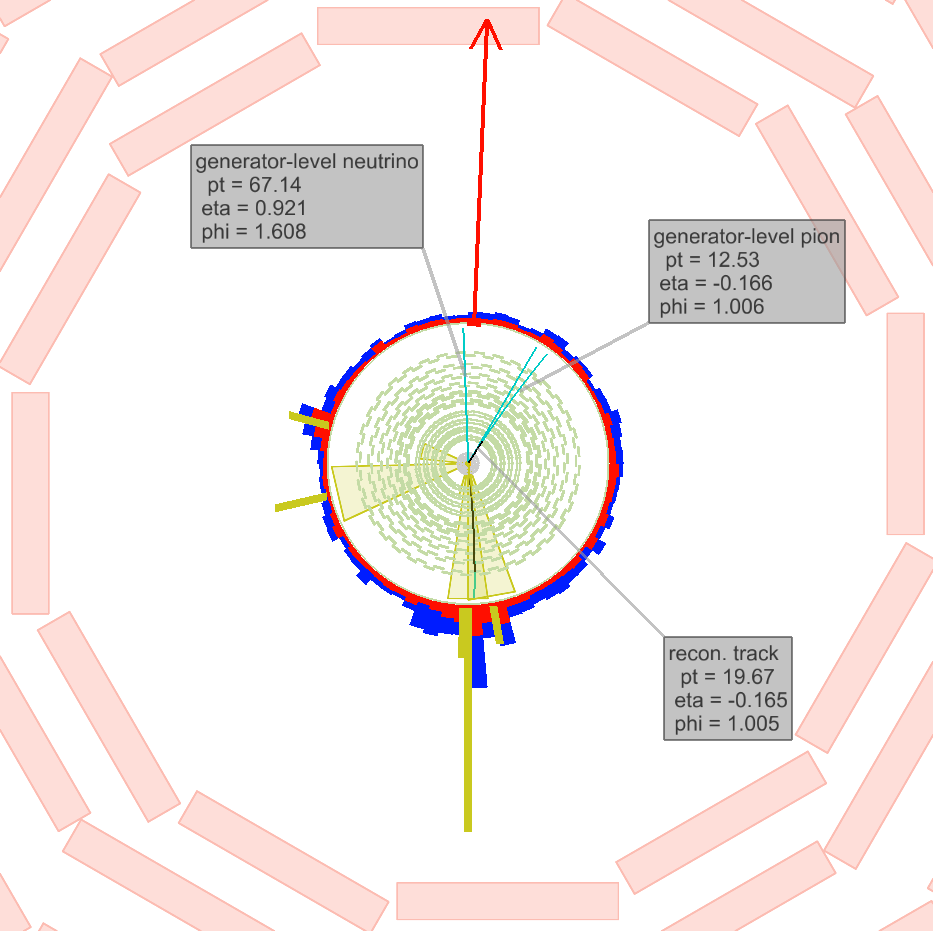
\includegraphics[width=0.49\textwidth]{figures/analysis/LostTau_Lumi_60133_Event_24033837.png}
  \end{tabular}
  \caption{Visualisation of a $W^{+}\rightarrow \tau^{+}\nu_{\tau} \rightarrow \pi^{+}\bar{\nu}_{\tau} \nu_{\tau} $ event contributing to the SM background. 
           In light blue the generator-level particles $\pi^{+}$, $\bar{\nu}_{\tau}$ and $\nu_{\tau}$ are shown.
           The reconstructed track (black line) is very short because the pion interacts with the tracker material via the strong force.
           No corresponding ECAL or HCAL energy deposits are measured. Therefore the reconstruction of the pion failed.}
  \label{fig:LostTau}
\end{figure}

In~\cite{bib:CMS:DT_Thesis,bib:CMS:DT_8TeV_AN} events are rejected when the track is pointing in a region of $0.15<|\eta|<0.35$.
In this search, this cut was omitted to maximise signal acceptance. 
Due to the additional selection in \ias, muons can easily be efficiently suppressed.
E.g. in the event example shown in Fig~\ref{fig:LostMuon}, the muon has an \ias value of about 0.02.\\


In general, all leptons are minimal ionising.
However, as electrons are much lighter compared to muons or pions, they loose more energy also via radiative effects.
Still, all three lepton types loose much less energy compared to hypothetical new heavy particles.
To have the possibility to make an optimisation in the two main discriminating variables \pt and \ias, the background estimation methods are designed to work for all different \pt and \ias selection cuts.
A comparison of the \ias distribution for all four different background sources is shown in Fig~\ref{fig:IasDist}.
\begin{figure}[!tb]
  \centering 
  \vspace{25pt}
  \begin{tabular}{c}
    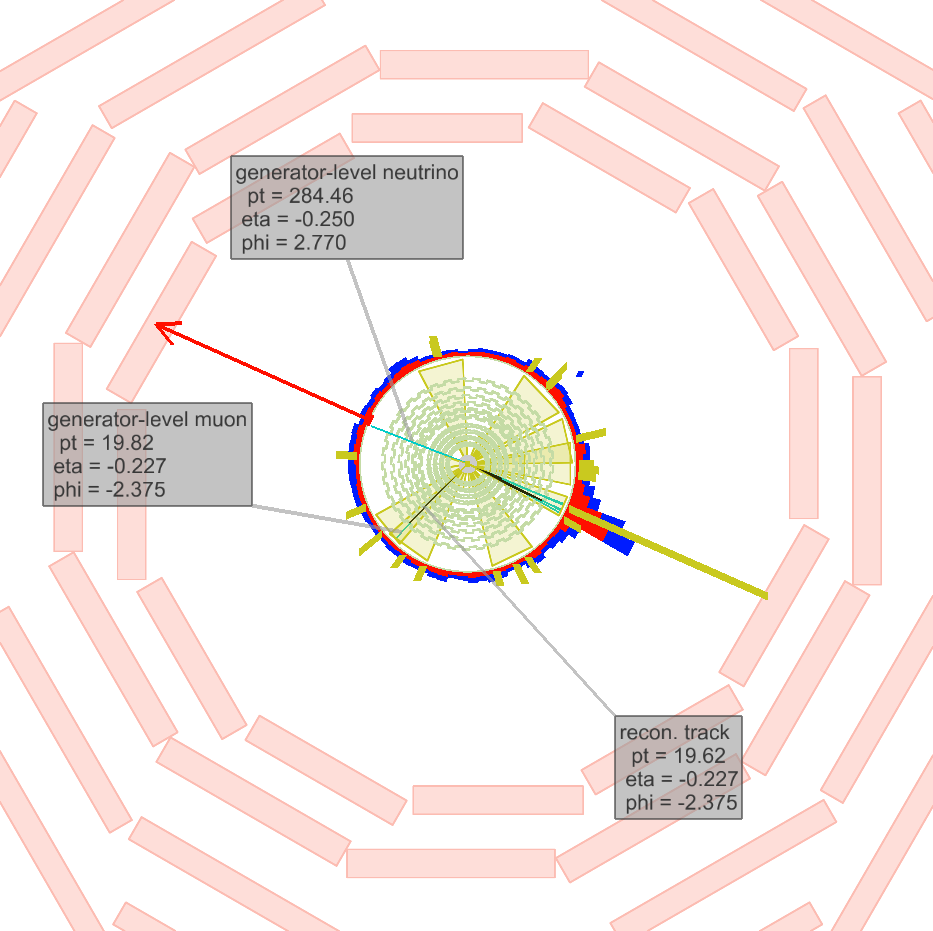
\includegraphics[width=0.49\textwidth]{figures/analysis/LostMuon_Lumi_357583_Event_142918834.png}
  \end{tabular}
  \caption{Visualisation of an $W\rightarrow \mu\nu_{\mu}$ event contributing to the SM background. 
           In light blue the generator-level particles $\mu$ and $\nu_{\mu}$ of the $W$ decay are shown. 
           The muon is pointing to the $\eta$-region between stations 0 and 1 of the DT system at $|\eta|\sim0.25$.
           In this region the muon reconstruction is less effcient. No signal in the muon chambers are visible. Therefore the  muon could not be reconstructed.}
  \label{fig:LostMuon}
\vspace{25pt}
\end{figure}

\begin{figure}[!tb]
  \centering 
  \vspace{25pt}
  \begin{tabular}{c}
    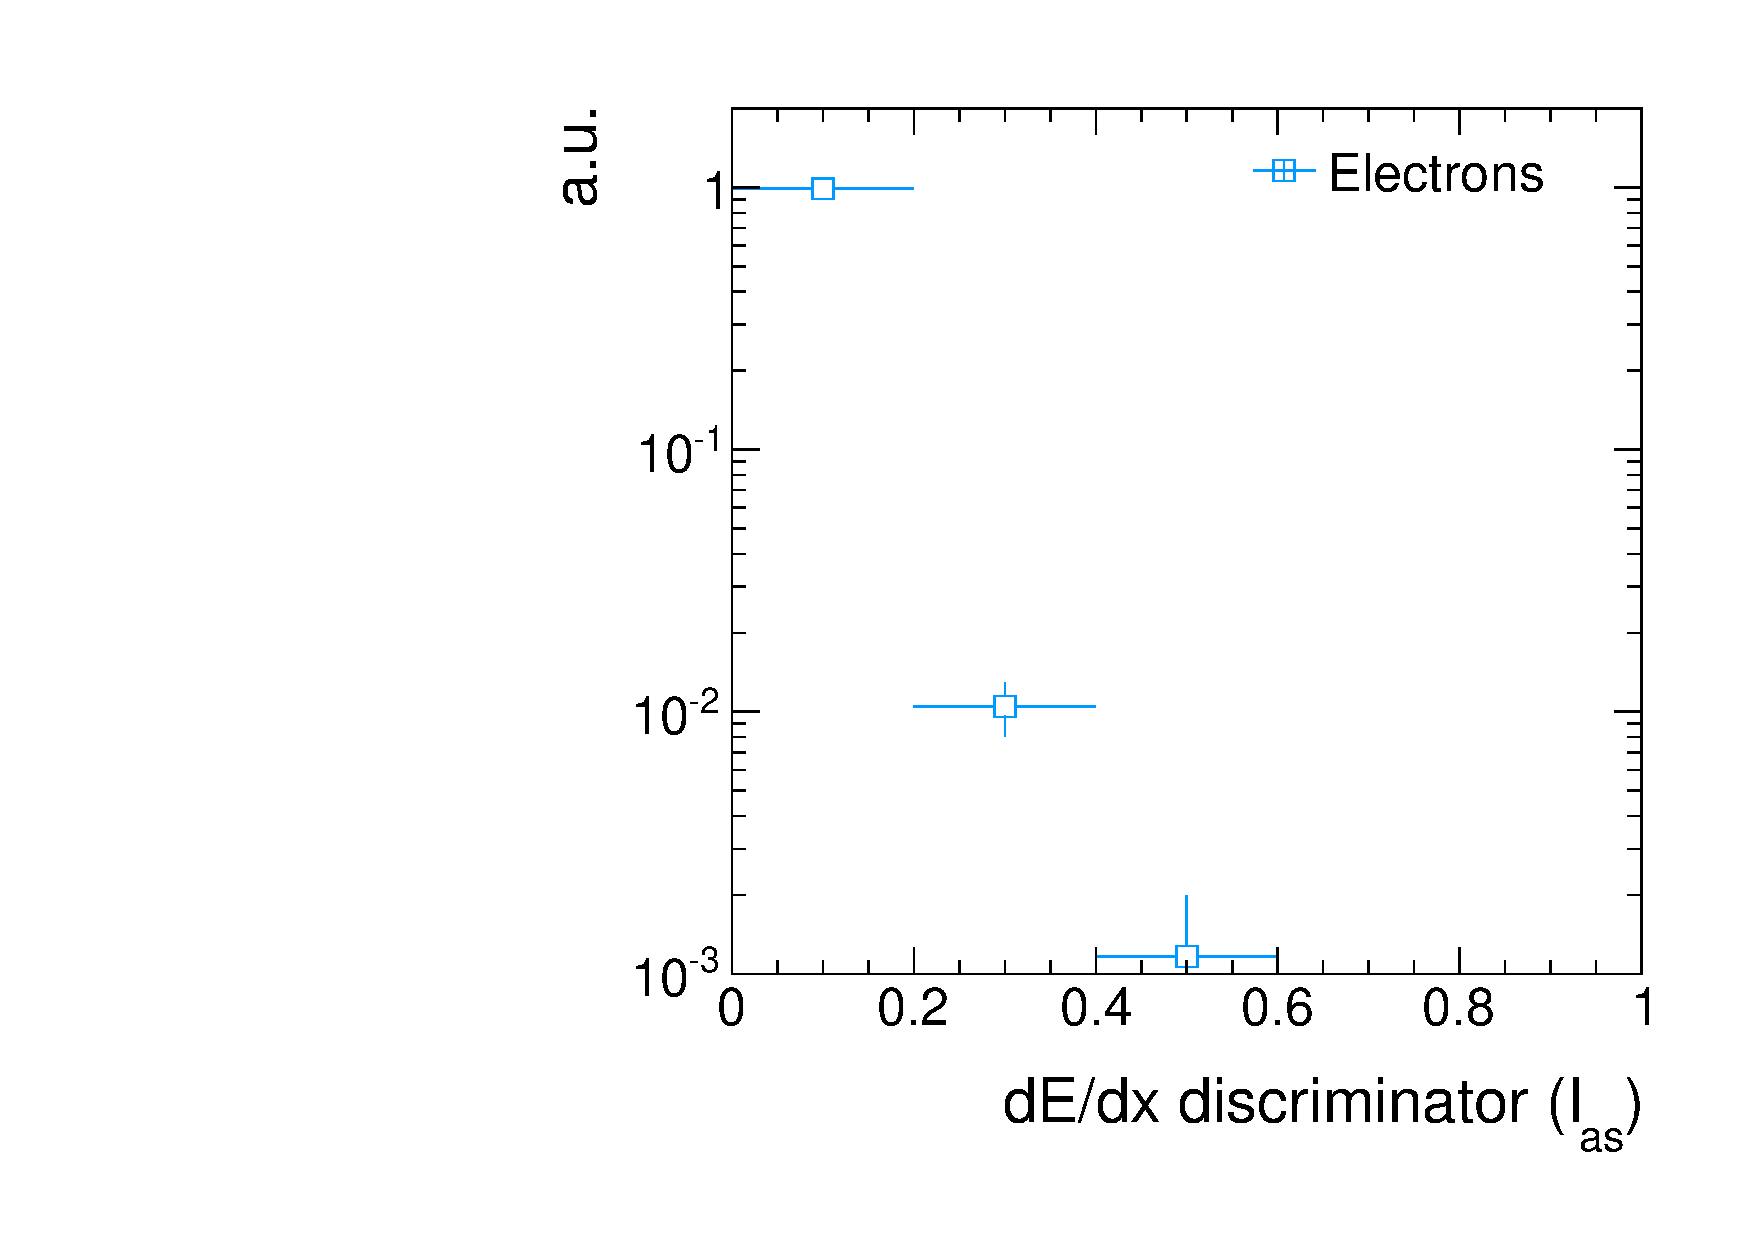
\includegraphics[width=0.33\textwidth]{figures/analysis/IasDistributionForElecs.pdf}
    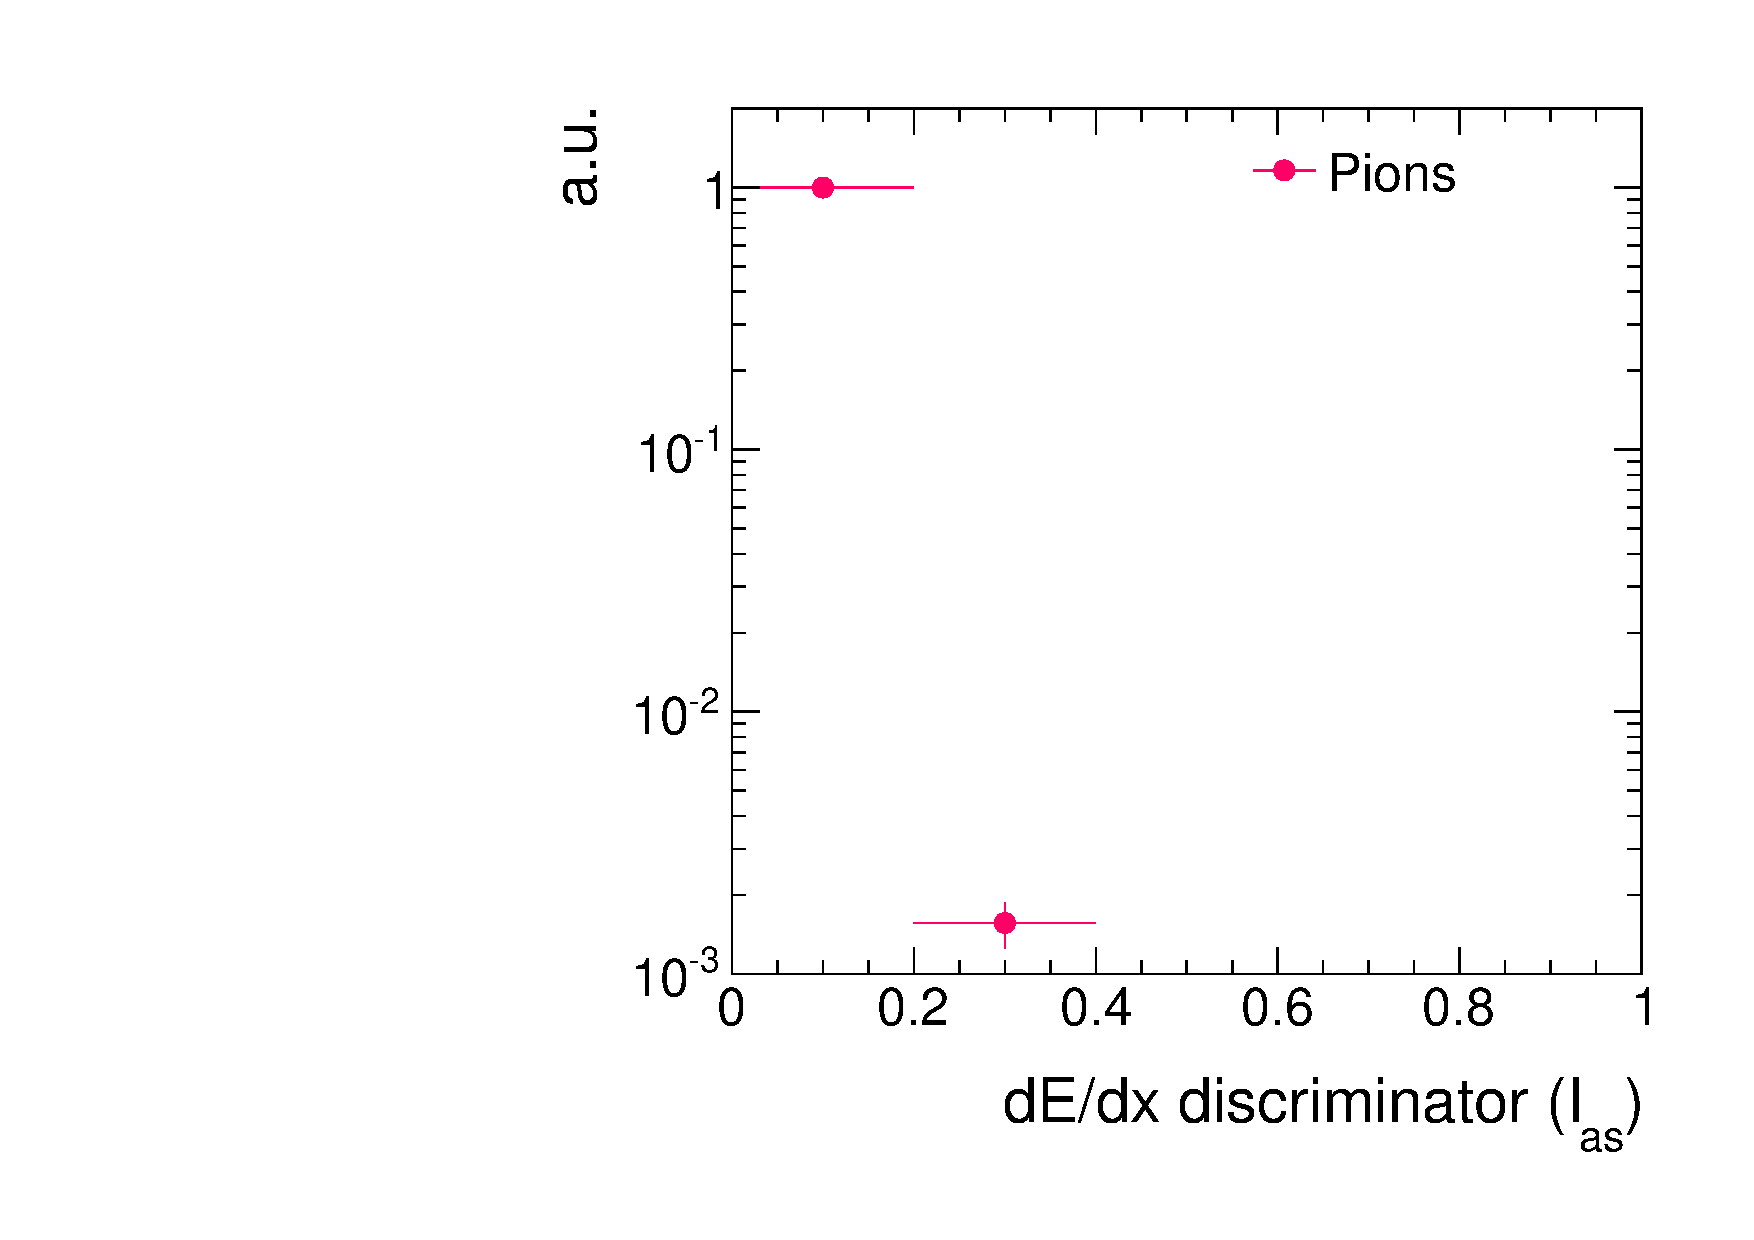
\includegraphics[width=0.33\textwidth]{figures/analysis/IasDistributionForPions.pdf}
    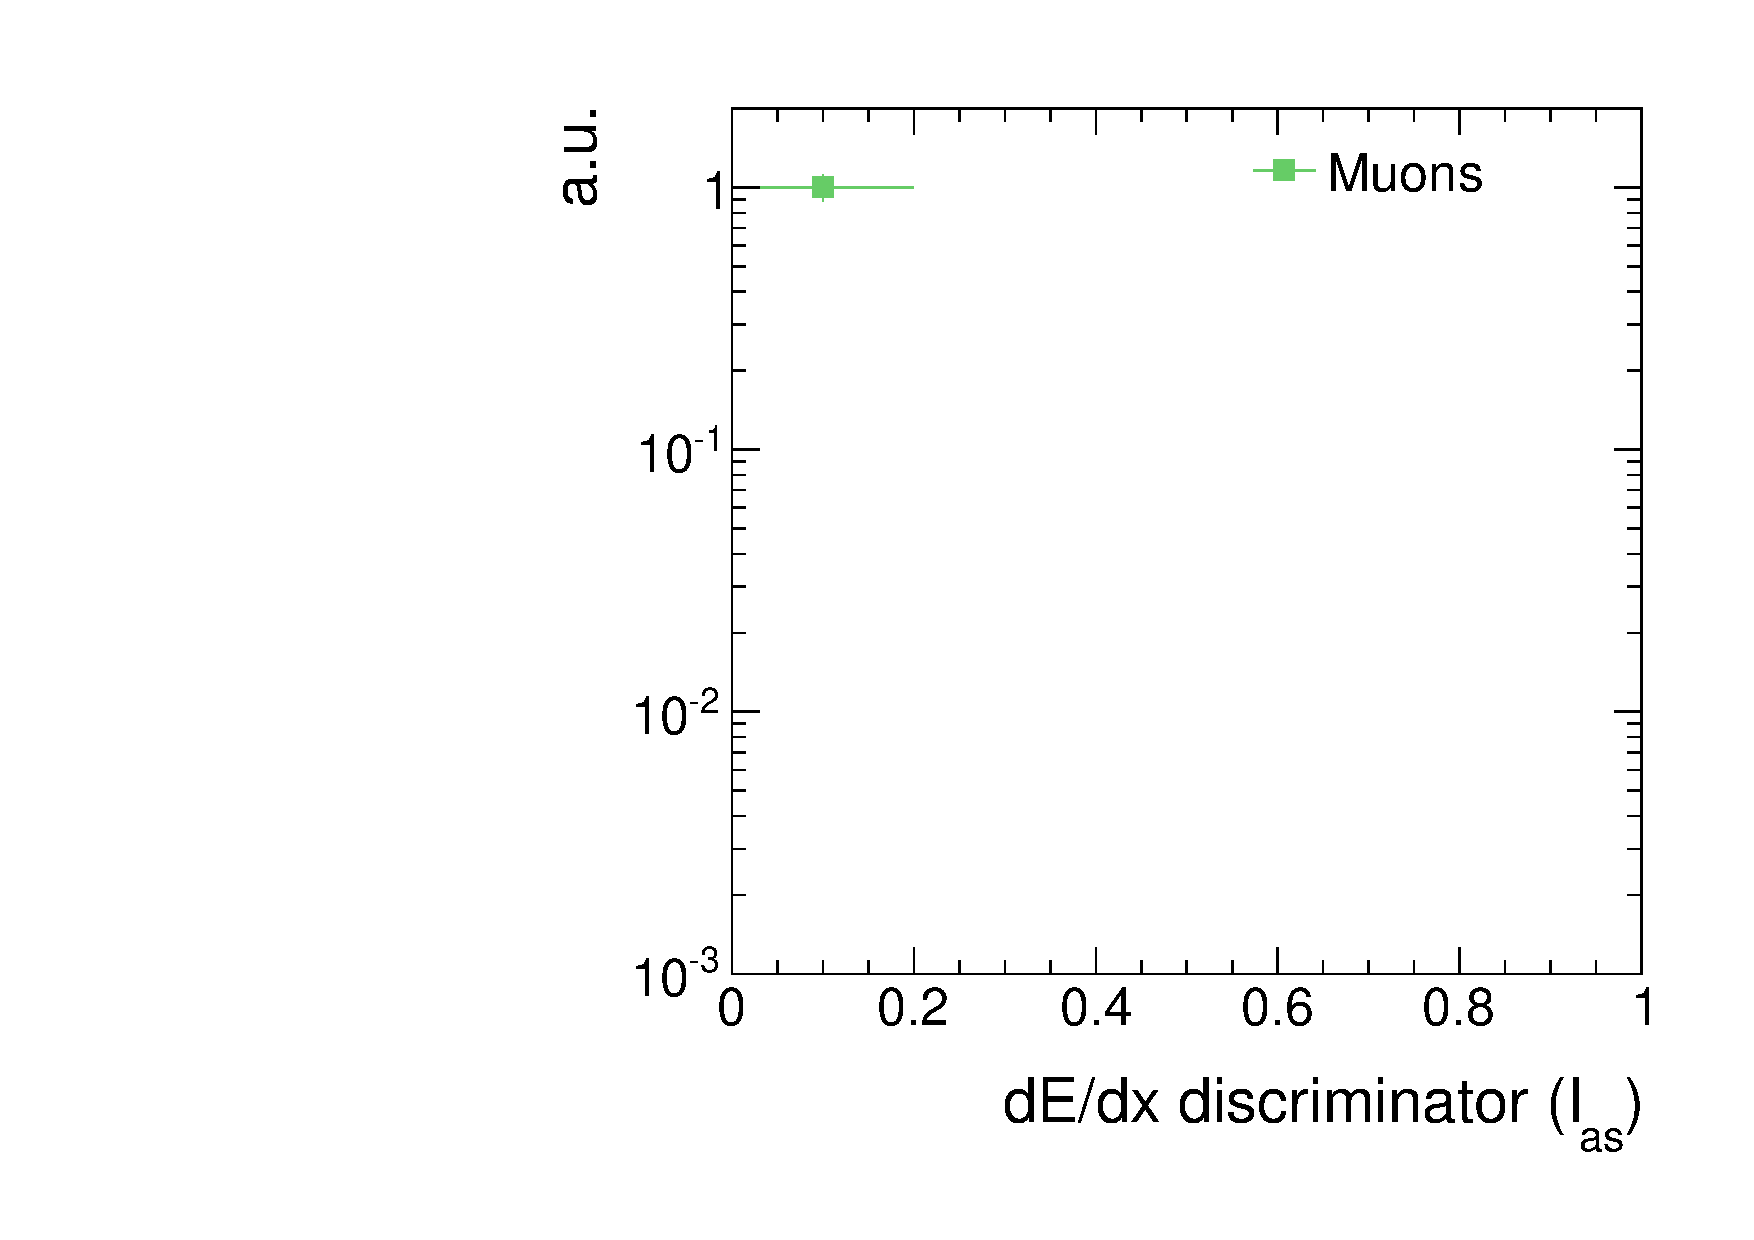
\includegraphics[width=0.33\textwidth]{figures/analysis/IasDistributionForMuons.pdf}
  \end{tabular}
  \caption{Normalised \ias distribution for electrons (left), pions (middle) and muons (right). 
           For all leptons the \ias distribution is rapidly falling.}
  \label{fig:IasDist}
\vspace{25pt}
\end{figure}


Again, also for the leptonic background the estimation method is splitted into two parts.
First, the estimation of the inclusive background without \ias information.
Second, the estimation of the \ias shape.


\subsection*{Inclusive leptonic background estimation}
The inclusive lepton background estimation is done with the help of leptonic control samples.
Blabl abla ba much more text is needed is needed is needed .
Blabl abla ba much more text is needed is needed is needed .
Blabl abla ba much more text is needed is needed is needed .
Blabl abla ba much more text is needed is needed is needed .
Blabl abla ba much more text is needed is needed is needed .
Blabl abla ba much more text is needed is needed is needed .
Blabl abla ba much more text is needed is needed is needed .
Blabl abla ba much more text is needed is needed is needed .
Blabl abla ba much more text is needed is needed is needed .
Blabl abla ba much more text is needed is needed is needed .
Blabl abla ba much more text is needed is needed is needed .
Blabl abla ba much more text is needed is needed is needed .


\section{Systematic uncertainties}
\label{sec:SysUncertaintiesBkg}


\begin{itemize}
\item Background consist of particles which make high energy deposits and are high pt
\item In general: Low background search
\end{itemize}
%%%%%%%%%%%%%%%%%%%%%%%%%%%%%%%%%%%%%%%%%%%%%%%%%%%%%%%%%%%%%%%%%%%%%%%%%%%%%%%%%%%%%%%%%%%%%%%%%%%%%%%%%%%%%%%%%%%%%%%%%%%%%%%%%%%%%%%%%%%%%%%%%%%%%%%%%%%%%%%%%%%%%%%%%%%%%%%%%%%%
%%%%%%%%%%%%%%%%%%%%%%%%%%%%%%%%%%%%%%%%%%%%%%%%%%%%%%%%%%%%%%%%%%%%%%%%%%%%%%%%%%%%%%%%%%%%%%%%%%%%%%%%%%%%%%%%%%%%%%%%%%%%%%%%%%%%%%%%%%%%%%%%%%%%%%%%%%%%%%%%%%%%%%%%%%%%%%%%%%%%
\chapter{Optimisation of search sensitivity}
\label{sec:Optimisation}
\begin{itemize}
\item Show plots
\item show table
\item Include NlostOuter here, too
\end{itemize}


%%%%%%%%%%%%%%%%%%%%%%%%%%%%%%%%%%%%%%%%%%%%%%%%%%%%%%%%%%%%%%%%%%%%%%%%%%%%%%%%%%%%%%%%%%%%%%%%%%%%%%%%%%%%%%%%%%%%%%%%%%%%%%%%%%%%%%%%%%%%%%%%%%%%%%%%%%%%%%%%%%%%%%%%%%%%%%%%%%%%
\chapter{Results}
\label{sec:Results}
\begin{itemize}
\item Data cutflowtable
\item Tables with results
\item One plot (4 bins: Prediction and data)
\end{itemize}

%%%%%%%%%%%%%%%%%%%%%%%%%%%%%%%%%%%%%%%%%%%%%%%%%%%%%%%%%%%%%%%%%%%%%%%%%%%%%%%%%%%%%%%%%%%%%%%%%%%%%%%%%%%%%%%%%%%%%%%%%%%%%%%%%%%%%%%%%%%%%%%%%%%%%%%%%%%%%%%%%%%%%%%%%%%%%%%%%%%%
\chapter{Interpretation}
\label{sec:Interpretation}
\section{Systematic uncertainties of simulated signal samples}
\section{Statistical Methods/ Limit setting}
\section{Exclusion limits}
\begin{itemize}
\item 1-d limits
\item 2-d limits
\end{itemize}

